\documentclass{article}
\usepackage{graphicx}
\usepackage[utf8]{inputenc}
\usepackage{latexsym,amsfonts,amssymb,amsthm,amsmath}
\usepackage[a4paper,margin=1in]{geometry} % Adjust margins as needed
\usepackage{float}
\usepackage{hyperref}


\setlength{\parindent}{0in}
\setlength{\oddsidemargin}{0in}
\setlength{\textwidth}{6.5in}
\setlength{\textheight}{8.8in}
\setlength{\topmargin}{0in}
\setlength{\headheight}{18pt}




\begin{document}

	\begin{titlepage}
    	\vspace*{\fill} % Add space before the title block
    	\begin{center}
        	{\huge \textbf{CMU Fall24 16820 Homework 1} \par}
       		\vspace{0.5cm}
        		{\large Patrick Chen \par}
        		\vspace{0.5cm}
		{\large Collaborators: \par}
		\vspace{0.5cm}
        		{\large September 7, 2024 \par}
    	\end{center}
    	\vspace*{\fill} % Add space after the title block to center everything
	\end{titlepage}
	
	\newpage
	\subsection*{Q1.1 at page 2}
	Ans:\\
	\hangindent=1.5em \hspace{1.5em} Given two camera projection matrices $P_1$ and $P_2$ corresponding to two cameras: camera 1 and camera 2, I have the following equations (1) and equations (2), where $x_1$ represents the projected 2D point, on the image plane of camera 1, of a 3D point, $x_\pi$, from a different 3D plane $\pi$, and $x_2$ represents the projected 2D point of the same 3D point, $x_\pi$, on the image plane of camera 2. 
	\begin{equation}
		x_1 = P_1 x_\pi
	\end{equation}
		\begin{equation}
		x_2 = P_2 x_\pi
	\end{equation}
	Both of equation (1) and (2) has the same 3D point $x_\pi$, it leads to the following equation (3):
	\begin{equation}
		P_1^{-1}x_1 = P_2^{-1} x_2
	\end{equation}
	Then I move $P_1$ to the right hand side by both multiply $P_1$ in equation (1) and (2), then I got equation (4).
	\begin{equation}
		x_1 = P_1 P^{-1}_2 x_2
	\end{equation}
	It is the same form of the given equation (1) at page 2, which is the equation (5) here, where $\lambda$ is a scale:
	\begin{equation}
		x_1 = \lambda H x_2
	\end{equation}
	So I get equation (6):
	\begin{equation}
		H = \lambda P_1 P_2^{-1}
	\end{equation}
	Consequently, if I need to prove that H does exist, I need to prove that $P_2^{-1}$ does exist.
	As $x_\pi$ lies on a plane, it only has two degrees of freedom, and can be represented as a 2D point. So the projection matrix $P_1$ and $P_2$ can be reduced to simplified 3x3 Homography matrix $H_1$ and $H_2$, since the Z dimension in 3D world coordinate of $x_\pi$ is no longer needed as the projection now is only 2D plane to 2D plane transformation. So it gives the following equation:
	\begin{equation}
		H = \lambda H_1 H_2^{-1}
	\end{equation}
	Under this 2D plane to 2D plan transformation, the Homography between camera plane and 2D plans, $\pi$, can be simply reduced to $KR$, where K is the intrinsic matrix of the camera, and R is the rotation matrix. It is because that the translation is no longer needed as the camera plane can always be rotated to be parallel to the 2D plane, $\pi$, and do the further intrinsic mapping. So $H_1 = K_1R_1$ and $H_2 = K_2R_2$, $H_2^{-1} = R_2^{-1}K_2^{-1}$. Because $K_2$ and $R_2$ are invertible, it makes $H_2$ is also invertible, so H does exist: $H = \lambda H_1 H_2^{-1}$ .
	
	
	\newpage
	\subsection*{Q1.2 at page 3}
	Ans:\\
	\begin{enumerate}
		\item h has 9 variables, but it only has 8 degrees of freedom. Specifically, h is the transformation of two 2D homogeneous coordinates, and if it is multiplied by a scale, $\lambda$, then the transformation equation still holds because of homogeneous coordinates. As a result, I have to add a constraint like setting the last element of h to be 1 or setting $\|h_2\|$ = 1, and it decreases the degree for freedom by 1. So, h has 8 degrees of freedom.
		 
		\item Since h has 8 unknowns, and each point pair can contribute to 2 equations for solving h, I need 4 pairs of points to solve h.
    	\item Substitute the given equation of $\mathbf{x}_1^i \equiv H \mathbf{x}_2^i \quad (i \in \{1 \dots N\})$ with variables:\\
		\[
			\begin{bmatrix}
				x^i_1 \\
				y^i_1 \\
				1
			\end{bmatrix}
			=
			\begin{bmatrix}
			h_{11} & h_{12} & h_{13} \\
			h_{21} & h_{22} & h_{23} \\
			h_{31} & h_{32} & h_{33}
			\end{bmatrix}
			\begin{bmatrix}
				x^i_2 \\
				y^i_2 \\
				1
			\end{bmatrix}
		\]
		Then, I expand the equations to get:\\
		\begin{align*}
			x_1^i &= h_{11} x_2^i + h_{12} y_2^i + h_{13} \\
			y_1^i &= h_{21} x_2^i + h_{22} y_2^i + h_{23} \\
			1 &= h_{31} x_2^i + h_{32} y_2^i + h_{33}
		\end{align*}
		By dividing the last element of homogeneous coordinates to get real plane coordinates, I get the following two equations:
		\[
			x^i_1 = \frac{h_{11}x^i_2 + h_{12}y^i_2 + h_{13}}{h_{31}x^i_2 + h_{32}y^i_2 + h_{33}}
		\]
		\[
			y^i_1 = \frac{h_{21}x^i_2 + h_{22}y^i_2 + h_{23}}{h_{31}x^i_2 + h_{32}y^i_2 + h_{33}}
		\]
		Though multiplying through by denominator and then  rearrange:
		\begin{align*}
			h_{11}x^i_2 + h_{12}y^i_2 + h_{13} - h_{31}x^i_2x^i_1 - h_{32}y^i_2x^i_1 - h_{33}x^i_1 = 0 \\
			h_{21}x^i_2 + h_{22}y^i_2 + h_{23} - h_{31}x^i_2y^i_1 - h_{32}y^i_2y^i_1 - h_{33}y^i_1 = 0
		\end{align*}
		Then I rearrange it to fit into the matrix form $A_i h$ = 0
		\[
		\begin{bmatrix}
			x_2^i & y_2^i & 1 & 0 & 0 & 0 & -x_1^i x_2^i & -x_1^i y_2^i & -x_1^i \\
			0 & 0 & 0 & x_2^i & y_2^i & 1 & -y_1^i x_2^i & -y_1^i y_2^i & -y_1^i
		\end{bmatrix}
		\begin{bmatrix}
			h_{11} \\
			h_{12} \\
			h_{13} \\
			h_{21} \\
			h_{22} \\
			h_{23} \\
			h_{31} \\
			h_{32} \\
			h_{33}
		\end{bmatrix}
		=
		\begin{bmatrix}
			0 \\
			0 \\
			0 \\
			0 \\
			0 \\
			0 \\
			0 \\
			0 \\
			0
		\end{bmatrix}
		\]
		Then I derive $A_i$:
		\[
		A_i = \begin{bmatrix}
			x_2^i & y_2^i & 1 & 0 & 0 & 0 & -x_1^i x_2^i & -x_1^i y_2^i & -x_1^i \\
			0 & 0 & 0 & x_2^i & y_2^i & 1 & -y_1^i x_2^i & -y_1^i y_2^i & -y_1^i
		\end{bmatrix}
		\]
		\item 
			\begin{enumerate}
				\item A trivial solution for h is all 0: 
				\[
				h = \begin{bmatrix}
					0 \\
					0 \\
					0 \\
					\vdots \\
					0
				\end{bmatrix}
				\]
				\item A is not full rank. In homogeneous system, if h is not trivial, then A must not be invertible, or the only solution of h would be a zero vector (trivial). It means that A should be singular, in other words, A must not be full rank.
				\item The impact of A being not full rank is that the smallest singular values would be zero or near zero, allowing to find a non-trivial solution h.
			\end{enumerate}
	\end{enumerate}

	\newpage
	\subsection*{Q1.4.1 at page 4}
	Ans:\\
	\hangindent=1.5em \hspace{1.5em} Given two cameras separated by a pure rotation, I have the following two equations:
	\begin{equation}
		x_1 = K_1 I X
	\end{equation}
	\begin{equation}
		x_2 = K_2 R X
	\end{equation}
	Since X is the same data point in 3D space, then I can substitute X in equation (7) with X in equation (8) and result in the following equation:
	\begin{equation}
		x_1 = K_1 R^{-1} K_2^{-1} x_2
	\end{equation}
	Since $x_1 = \lambda H x_2$, then I can know that:
	\begin{equation}
		H = \frac{1}{\lambda} K_1 R^{-1} K_2^{-1}
	\end{equation}
	Since $K_2$ and $R$ are invertible, $\det(K_2) \neq 0$ and $\det(R) \neq 0$, H does exist.
	
	\newpage
	\subsection*{Q1.4.2 at page 4}
	Ans:\\
	\hangindent=1.5em \hspace{1.5em} Recall from Q1.4.1, $H = K_1R(\theta)^{-1}K_2^{-1}$, given that $\theta$ is the angle of rotation. Since $K_1=K_2=K$, I have:
	\begin{equation}
		H = K R(\theta)^{-1} K^{-1}
	\end{equation}
	By multiplying two H together:
	\begin{equation}
		H^2 = (K R(\theta)^{-1} K^{-1})  (K R(\theta)^{-1} K^{-1})
	\end{equation}
	By removing redundant identity matrix:
	\begin{equation}
		H^2 = K R(\theta)^{-1} R(\theta)^{-1} K^{-1}
	\end{equation}
	According to the property of rotation matrix $R(\theta)^{-1}=R(\theta)^T=R(-\theta)$, and $R(-\theta) R(-\theta) = R(-2\theta)$, I have $R(\theta)^{-1} R(\theta)^{-1} = R(2\theta)^{-1}$, so I have:
	\begin{equation}
		H^2 = K R(2\theta)^{-1} K^{-1}
	\end{equation}
	It demonstrates that $H^2$ corresponds to a rotation of $2\theta$.
	
	\newpage
	\subsection*{Q1.4.3 at page 4}
	Ans:\\
	\hangindent=1.5em \hspace{1.5em} It is because that either one of the following two conditions is needed to be held for the planar homography to exist:
	\begin{enumerate}
		\item The points in the 3D world lie on a 2D plane.
		\item Only pure rotation between two views.
	\end{enumerate}
	\hangindent=1.5em \hspace{1.5em} As a result, planar homography is not completely sufficient to map any scene image to another viewpoint.
	
	\newpage
	\subsection*{Q1.4.4 at page 5}
	Ans:\\
	\hangindent=1.5em \hspace{1.5em} The projection matrix P is a $3\times4$ matrix that can map a 3D point, X, to a 2D point, x:
	\begin{equation}
		x = P X
	\end{equation}
	A line in 3D space can be represented as the following equation, where t is a parameter:
	\begin{equation}
		X(t) = X_1 + t(X_2-X_1) 
	\end{equation}
	If I multiply the projection matrix, P, on both hand sides of equation (16), then I have:
	\begin{equation}
		P X(t) = P X_1 + t P (X_2-X_1) 
	\end{equation}
	By moving P into parenthesis, then:
	\begin{equation}
		P X(t) = P X_1 + t (P X_2- P X_1) 
	\end{equation}	
	Then, I got the following equation:
	\begin{equation}
		x(t) = x_1 + t (x_2- x_1) 
	\end{equation}
	Equation (19) is the equation of line on a 2D plane. As a result, the line can be preserved through perspective projection P.	
	
	\newpage
	\subsection*{Q2.1.1 at page 5}
	Ans:\\
	\hangindent=1.5em \hspace{1.5em} FAST detector has the following differences when comparing with Harris corner detector:
	\begin{enumerate}
		\item FAST detector is not rotation-invariant, while Harris corner detector can be rotation-invariant with some tricky implementation details.		
		\item FAST detector only compare intensities with neighbors in a circular range around a candidate point, while Harris corner detector uses much more expansive computations like first order derivative (gradient), summation of a window of gradients, and solving eigenvalue problems, leading to the result that FAST detector is much more faster than Harris corner detector.
		\item FAST detector is more sensitive to noise and the change of lighting, while Harris corner detector is more robust to noise and lighting change because Harris corner detector gets more information from gradients in multiple directions of a window plus solving eigenvalue problems to get optimized candidates of corners.
		\item FAST detector is faster but less accurate in the localizing features, while Harris corner detector is slower but more accurate in localizing feature points.
	\end{enumerate}
	
	\newpage
	\subsection*{Q2.1.2 at page 5}
	Ans:\\
	\hangindent=1.5em \hspace{1.5em} BRIEF descriptor has the following differences when comparing with filterbanks descriptor:
	\begin{enumerate}
		\item BRIEF descriptor chooses n pairs of points within a predefined window to form a n-bit binary descriptor by setting each bit 1 or 0 according to the comparison of each pair of selected points, while filterbanks convolve the image with a series of predefined filters to form an array of responses in each pixel as the descriptor.
		\item BREIF descriptor is faster than filterbanks descriptor as BRIEF descriptor only use sampling and comparison of intensity, while filterbanks descriptor applys convolution of different filters to produce different response as the descriptor. 
		\item As for the robustness, filterbanks descriptor is more robust to rotation and scale as it can apply different filters to mitigate the impact from scaling and rotating, while BRIEF descriptor only compares the intensity within a window and it is not rotation-invariant and scale-invariant. 
	\end{enumerate}
	
	\newpage
	\subsection*{Q2.1.3 at page 5}
	Ans:\\
	\hangindent=1.5em \hspace{1.5em} The Hamming distance is to calculate the number of different bits in two binary descriptors. For example, let $x_1$ be a d-dimensional binary descriptor: $x_1 = (x_1^0, x_1^1, ..., x_1^{(d-1)})$, and $x_2$ is another d-dimensional binary descriptor: $x_2 = (x_2^0, x_2^1, ..., x_2^{(d-1)})$, the Hamming distance is defined as the following:
	\begin{eqnarray}
		d_H(\mathbf{x_1}, \mathbf{x_2}) = \sum_{i=1}^{d} \delta(x_1^i, x_2^i), where\ \delta(x_1^i, x_2^i) =
		\begin{cases}
			0 & \text{if } x_1^i = x_2^i, \\
			1 & \text{if } x_1^i \neq x_2^i.
		\end{cases}
	\end{eqnarray}
	Hamming distance has the following benefits over conventional Euclidean distance measure:
	\begin{enumerate}
		\item Hamming distance is faster than Euclidean distance because Hamming distance only needs to compute the number of different bits among two binary vectors, and it can be computed by efficient XOR and counter operations, while Euclidean distance needs to compute several complex operations, like vector substraction, summation of square and square root operations, making Euclidean distance slow and expensive for computation.
		\item In our setting, I use BREIF descriptor on our detected feature points, resulting in vectors in binary form, and it is definitely suitable to use Hamming distance to compare two binary feature descriptor vectors. 
	\end{enumerate}
	
	\newpage
	\subsection*{Q2.1.4 at page 5}
	Ans:\\
	\hangindent=1.5em \hspace{1.5em} The best output is as the following Figure \ref{fig:best_output}, and the corresponding code snippets are as the following Figure \ref{fig:csn1}. The sigma is set to 0.08, and ration is set to 0.61.
	\begin{figure}[H]		
		\centering
		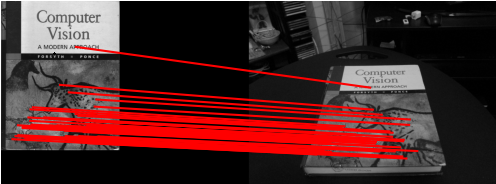
\includegraphics[width=0.8\textwidth]{Q2_1_4_best_output.png}  % Replace with your image file name
		\caption{Best Output}
		\label{fig:best_output}
	\end{figure}
	\begin{figure}[H]		
	\centering
	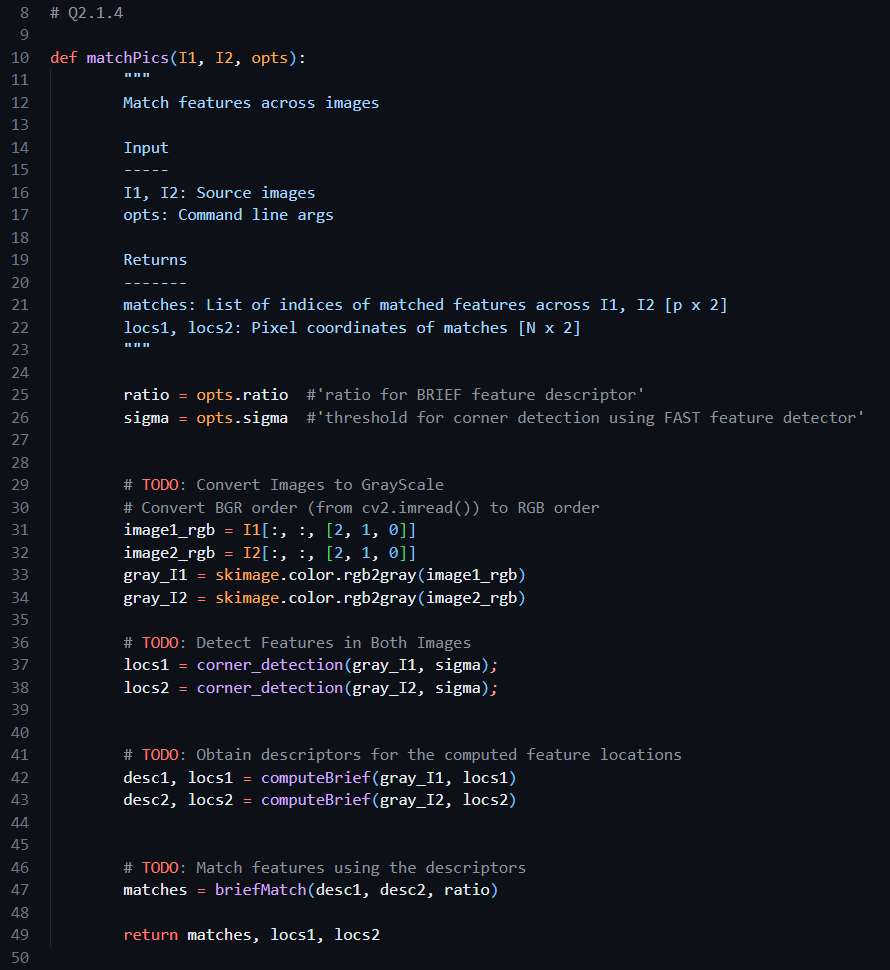
\includegraphics[width=\textwidth]{Q2_1_4_best_output_code1.png}  % Replace with your image file
	\caption{Q2.1.4 Code Snippet}
	\label{fig:csn1}
	\end{figure}
	
	\newpage
	\subsection*{Q2.1.5 at page 6}
	Ans:\\
	\hangindent=0.4em \hspace{0.3em} According to skimage API documentation, the sigma value is used in FAST detector to decide whether the pixels on the circle are brighter, darker, or similar with respect to the test pixel. The lower value of sigma would produce more detected feature points, while the higher value would produce less detected feature points. On the other hand, the ratio value is used in $skimage.feature.match\_descriptors()\ API$. It is the ratio between the distance of the first closest descriptors to the second closest descriptors. Thus, the higher the value would cause more matched correspondence as the matched condition is more easy, while the lower the value would cause less matched correspondence. The following experiments listed in Table \ref{table:exp} is started with the given values of sigma=0.15 and ratio=0.7. As I increase sigma, it results in more false positive matched points, such as the read line near the top of the image in row 1 and row 2 of Table \ref{table:exp}. So I decrease sigma to 0.10, and it shows up more unmatched points. Thus, I also decrease ratio to 0.65, and it shows less mismatched correspondence. As I decrease sigma to 0.08, and ratio to 0.61, I think I found the optimized result, as there is no mismatched correspondence. As I keep decreasing sigma to 0.7, the mismatched correspondence near the right border of the book in the right image shows up. As I decrease ratio from 0.61 to 0.55, the mismatched correspondence does not disappear. As the result, I think sigma=0.08 and ratio=0.61 is my best result.
	 
	\begin{table}[H]
		\centering
		\begin{tabular}{|c|c|c|}
			\hline
			\textbf{Parameter sigma} & \textbf{Parameter ratio} & \textbf{Generated Image} \\
			\hline
			0.20 & 0.7 & 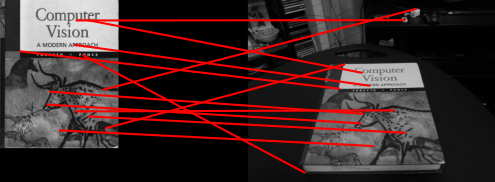
\includegraphics[width=0.4\textwidth]{Q2_1_4_0.20_0.7.png} \\
			\hline
			0.20 & 0.65 & 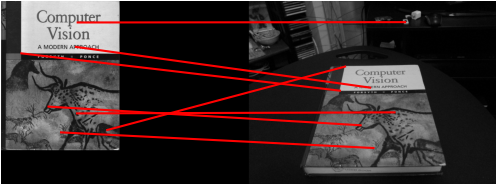
\includegraphics[width=0.4\textwidth]{Q2_1_4_0.20_0.65.png} \\						
			\hline
			0.15 & 0.7 & 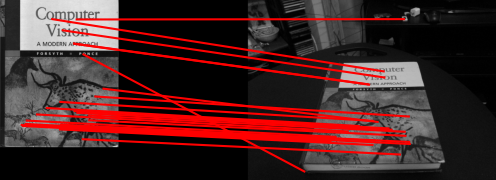
\includegraphics[width=0.4\textwidth]{Q2_1_4_0.15_0.7.png} \\
			\hline
			0.10 & 0.7 & 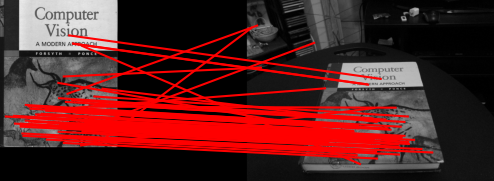
\includegraphics[width=0.4\textwidth]{Q2_1_4_0.10_0.7.png} \\			
			\hline
			0.10 & 0.65 & 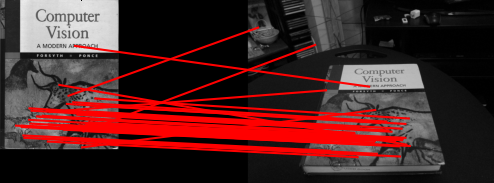
\includegraphics[width=0.4\textwidth]{Q2_1_4_0.10_0.65.png} \\
			\hline
			0.08 & 0.61 & 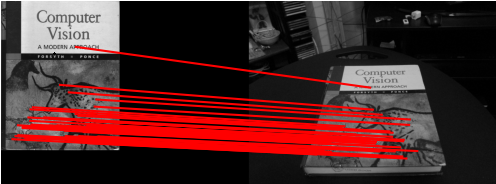
\includegraphics[width=0.4\textwidth]{Q2_1_4_best_output.png} \\
			\hline
			0.07 & 0.61 & 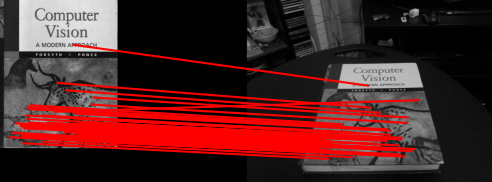
\includegraphics[width=0.4\textwidth]{Q2_1_4_0.07_0.61.png} \\
			\hline
			0.06 & 0.55 & 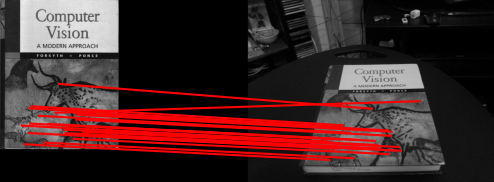
\includegraphics[width=0.4\textwidth]{Q2_1_4_0.06_0.55.png} \\
			\hline
		\end{tabular}
		\caption{Parameter Changes and Corresponding Generated Images}
		\label{table:exp}
	\end{table}

	\newpage
	\subsection*{Q2.1.6 at page 6}
	Ans:\\
	\hangindent=0.4em \hspace{0.3em} As shown in the Figure \ref{fig:hist_res}, the maximum of matches occurs at rotation = 0 degrees, and the rotation makes the number of matches decrease drastically. I think it is because the BRIEF descriptor and the FAST detector using in the matchPics() function is not rotation-invariant.
	
	\begin{figure}[H]		
		\centering
		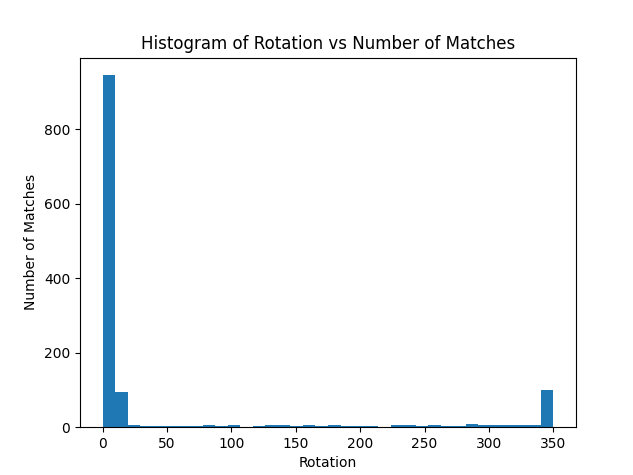
\includegraphics[width=0.8\textwidth]{Q2_1_6.png}  % Replace with your image file name
		\caption{Histogram Result}
		\label{fig:hist_res}
	\end{figure}	
	
	\begin{figure}[H]
	\centering
	\begin{minipage}[b]{0.45\textwidth}
		\centering
		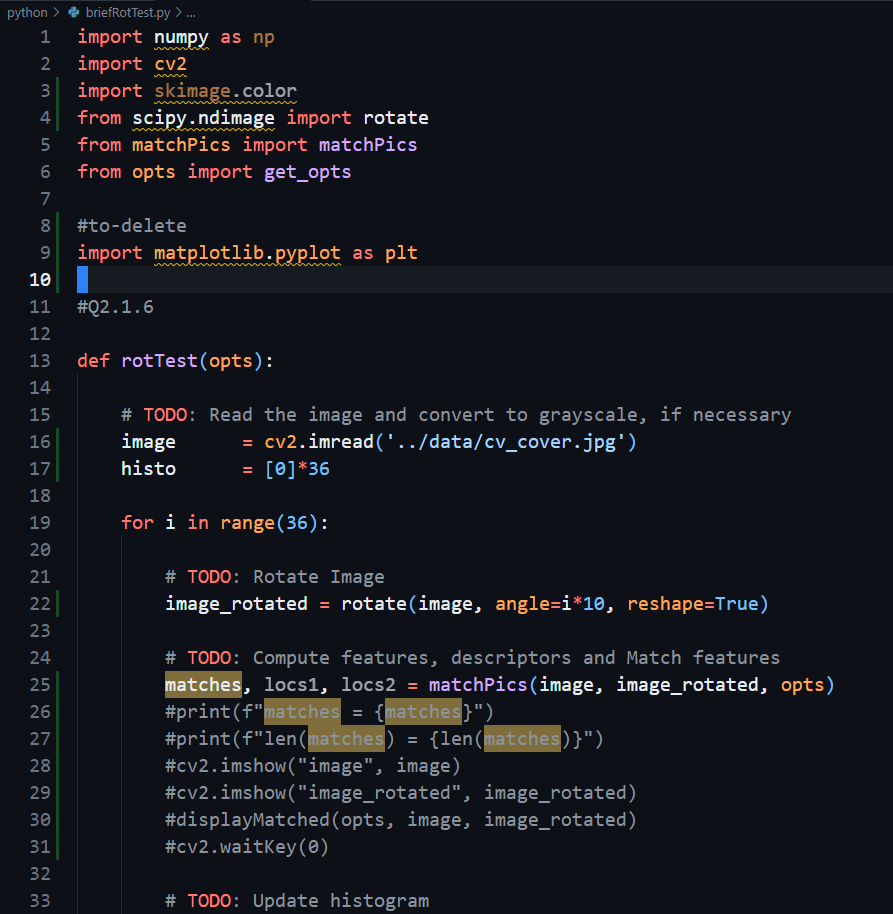
\includegraphics[width=\textwidth]{Q2_1_6_cns1.png}  % Replace with your image file
		\caption{Q2.1.6 Code Snippet 1}
		\label{fig:2_14_6_csn1}
	\end{minipage}
	\hfill  % This adds space between the images
	\begin{minipage}[b]{0.45\textwidth}
		\centering
		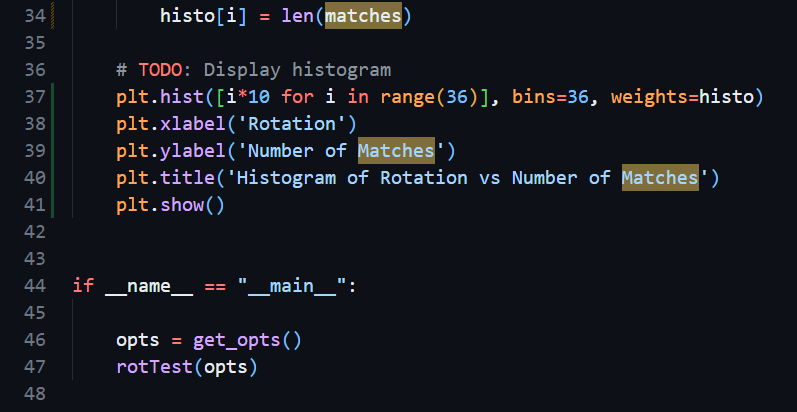
\includegraphics[width=\textwidth]{Q2_1_6_cns2.png}  % Replace with your image file
		\caption{Q2.1.6 Code Snippet 2}
		\label{fig:2_14_6_csn2}
	\end{minipage}
	\end{figure}
	
	\newpage
	\subsection*{Q2.1.7 at page 6}
	Ans:\\
	\hangindent=0.4em \hspace{0.3em} //to-do
	
	\newpage
	\subsection*{Q2.2.1 at page 7}
	Ans:\\
	\hangindent=0.4em \hspace{0.3em} Figure \ref{fig:Q221_cns} shows the code snippet.
	\begin{figure}[H]		
		\centering
		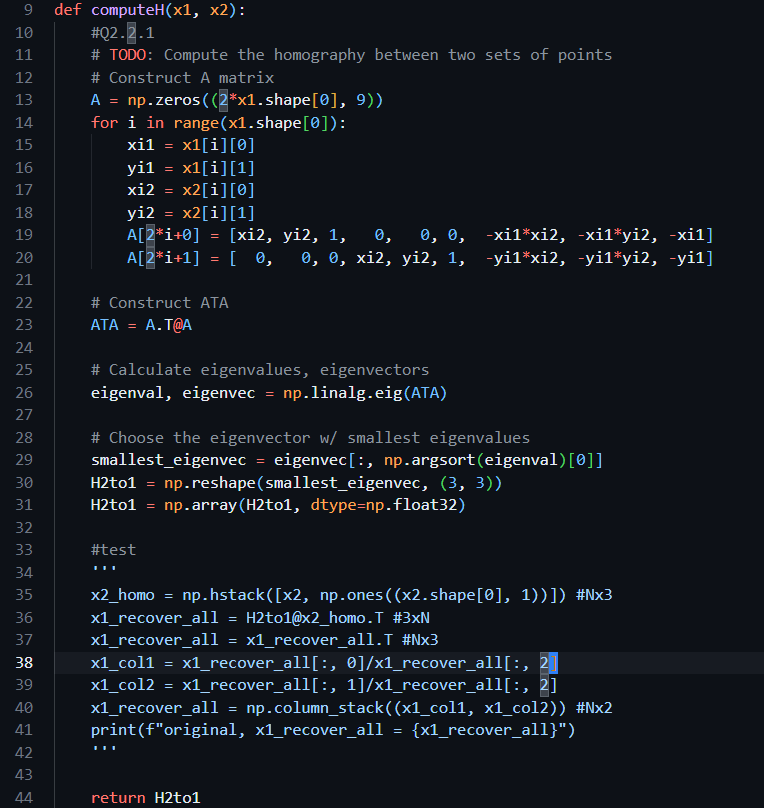
\includegraphics[width=0.8\textwidth]{Q2_2_1.png}  % Replace with your image file name
		\caption{Q2.2.1 Code Snippet}
		\label{fig:Q221_cns}
	\end{figure}
	
	\newpage
	\subsection*{Q2.2.2 at page 7}
	Ans:\\
	\hangindent=0.4em \hspace{0.3em} Figure \ref{fig:Q222_cns1} - Figure \ref{fig:Q222_cns3} show the code snippet.
	\begin{figure}[H]
	\centering
	\begin{minipage}[b]{0.45\textwidth}
		\centering
		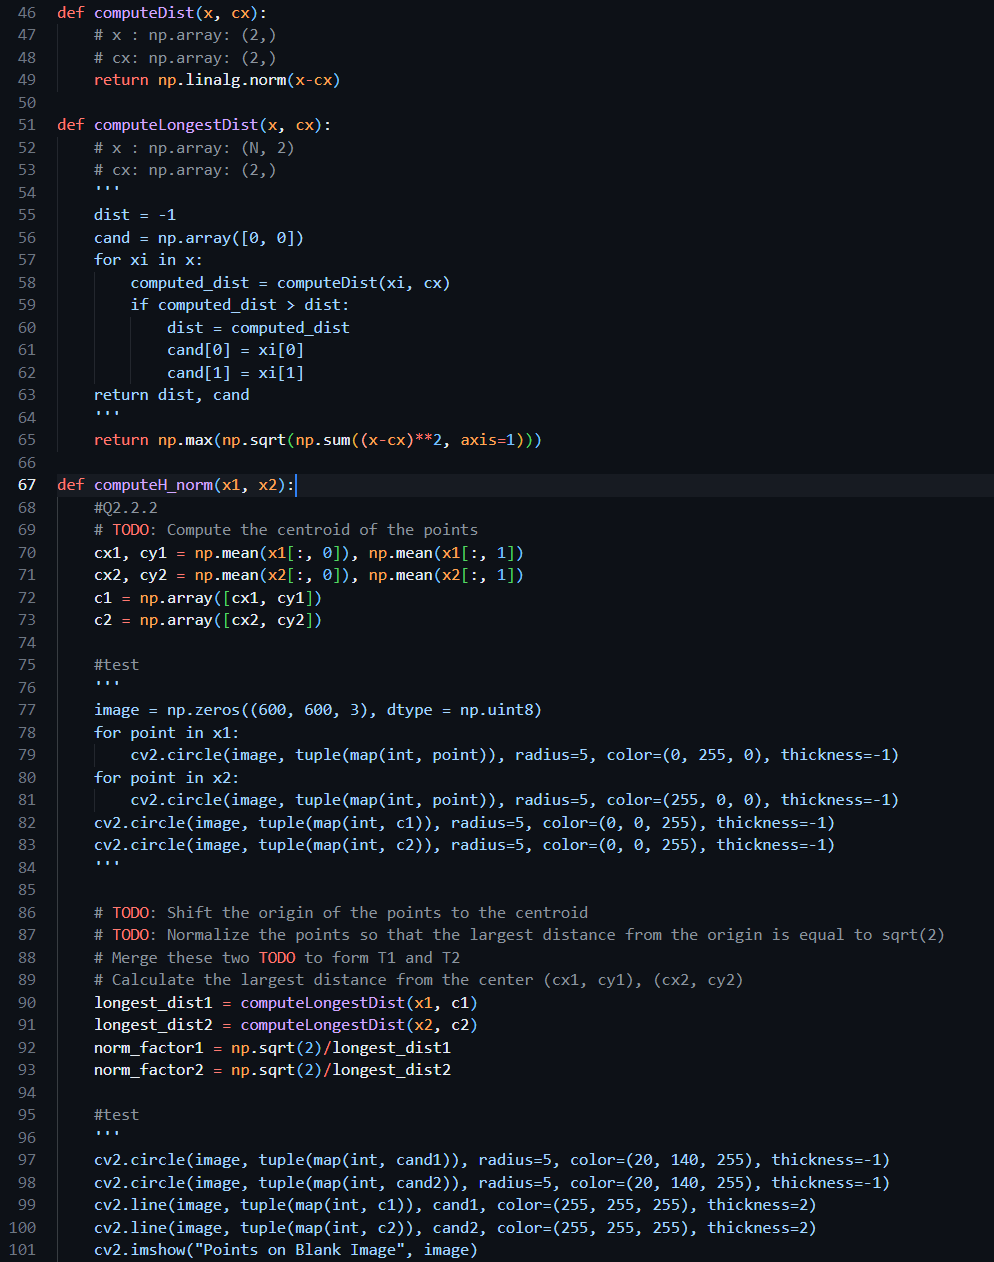
\includegraphics[width=\textwidth]{Q2_2_2_cns1.png}  % Replace with your image file
		\caption{Q2.2.2 Code Snippet 1}
		\label{fig:Q222_cns1}
	\end{minipage}
	\hfill  % This adds space between the images
	\begin{minipage}[b]{0.45\textwidth}
		\centering
		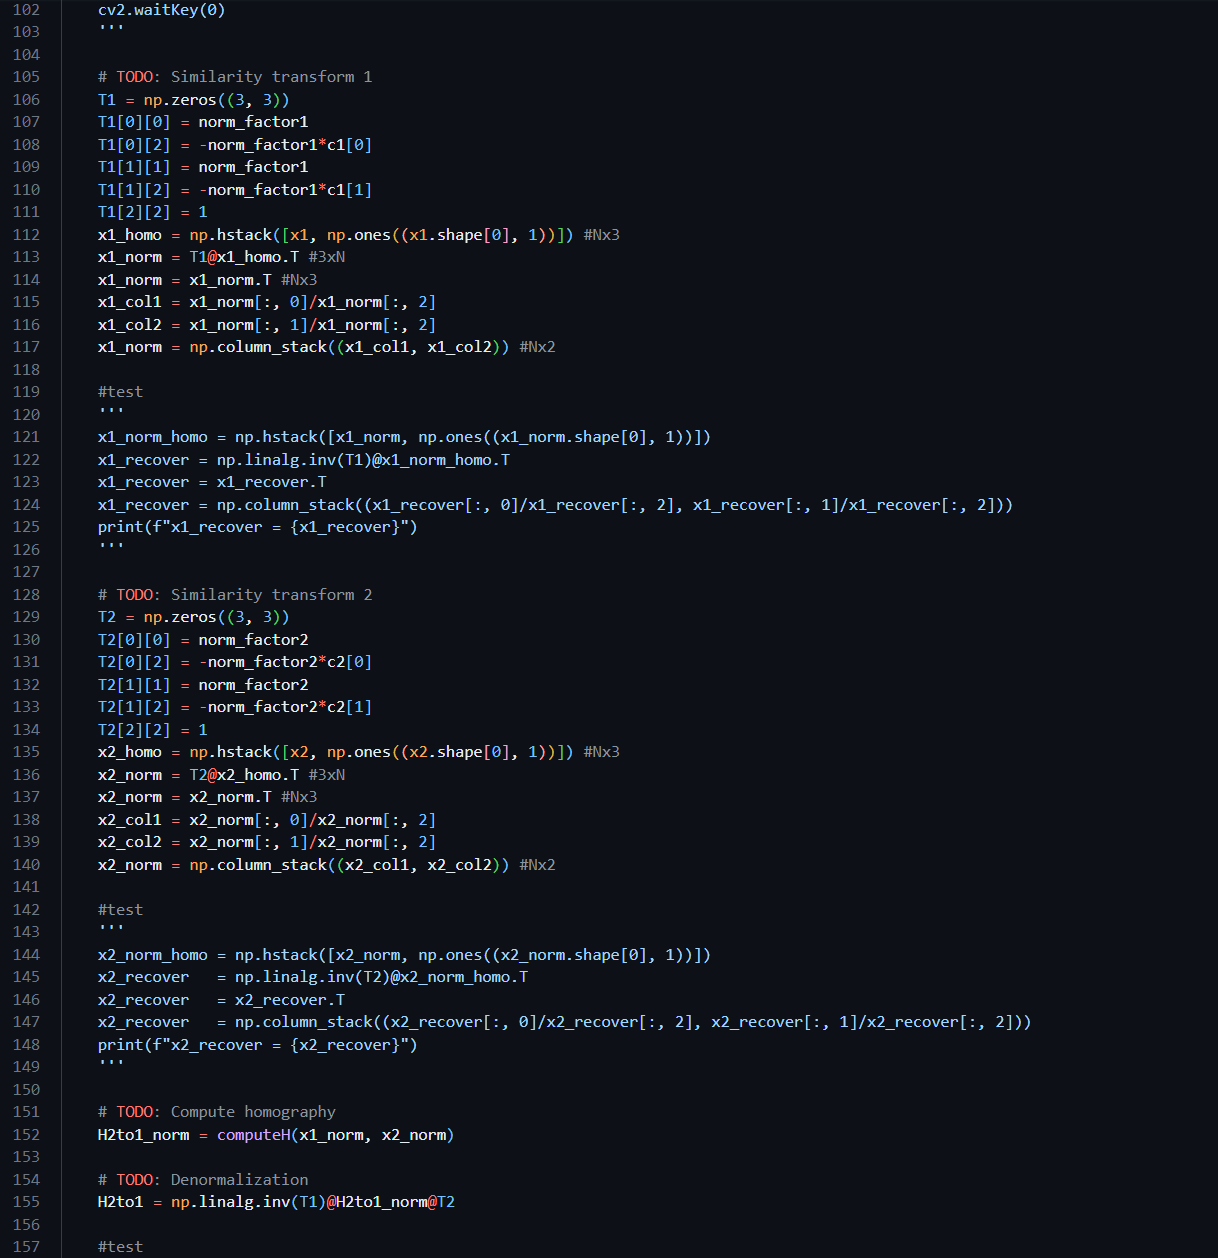
\includegraphics[width=\textwidth]{Q2_2_2_cns2.png}  % Replace with your image file
		\caption{Q2.2.2. Code Snippet 2}
		\label{fig:Q222_csn2}
	\end{minipage}
	\begin{figure}[H]		
		\centering
		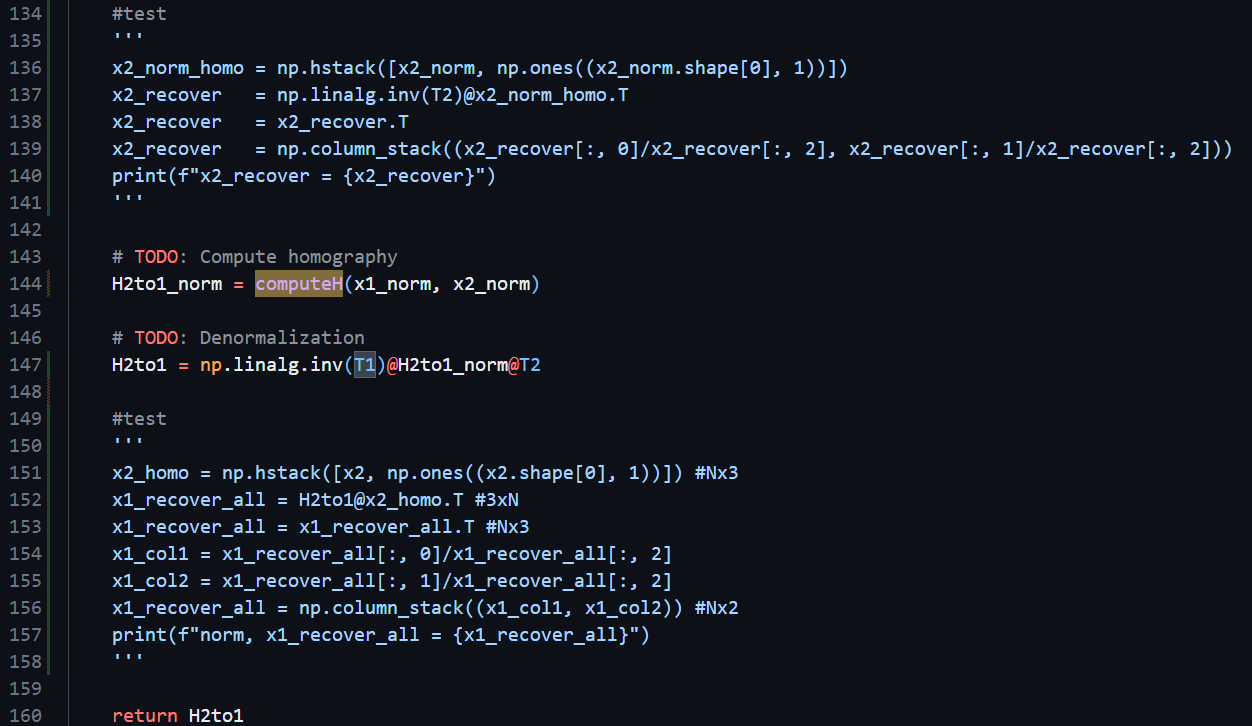
\includegraphics[width=0.8\textwidth]{Q2_2_2_cns3.png}  % Replace with your image file name
		\caption{Q2.2.2 Code Snippet3}
		\label{fig:Q222_cns3}
	\end{figure}	
	\end{figure}
	
	\newpage
	\subsection*{Q2.2.3 at page 7}
	Ans:\\
	\hangindent=0.4em \hspace{0.3em} Figure \ref{fig:Q223_cns1} - Figure \ref{fig:Q223_csn2} show the code snippet.
	\begin{figure}[H]
	\centering
	\begin{minipage}[b]{0.45\textwidth}
		\centering
		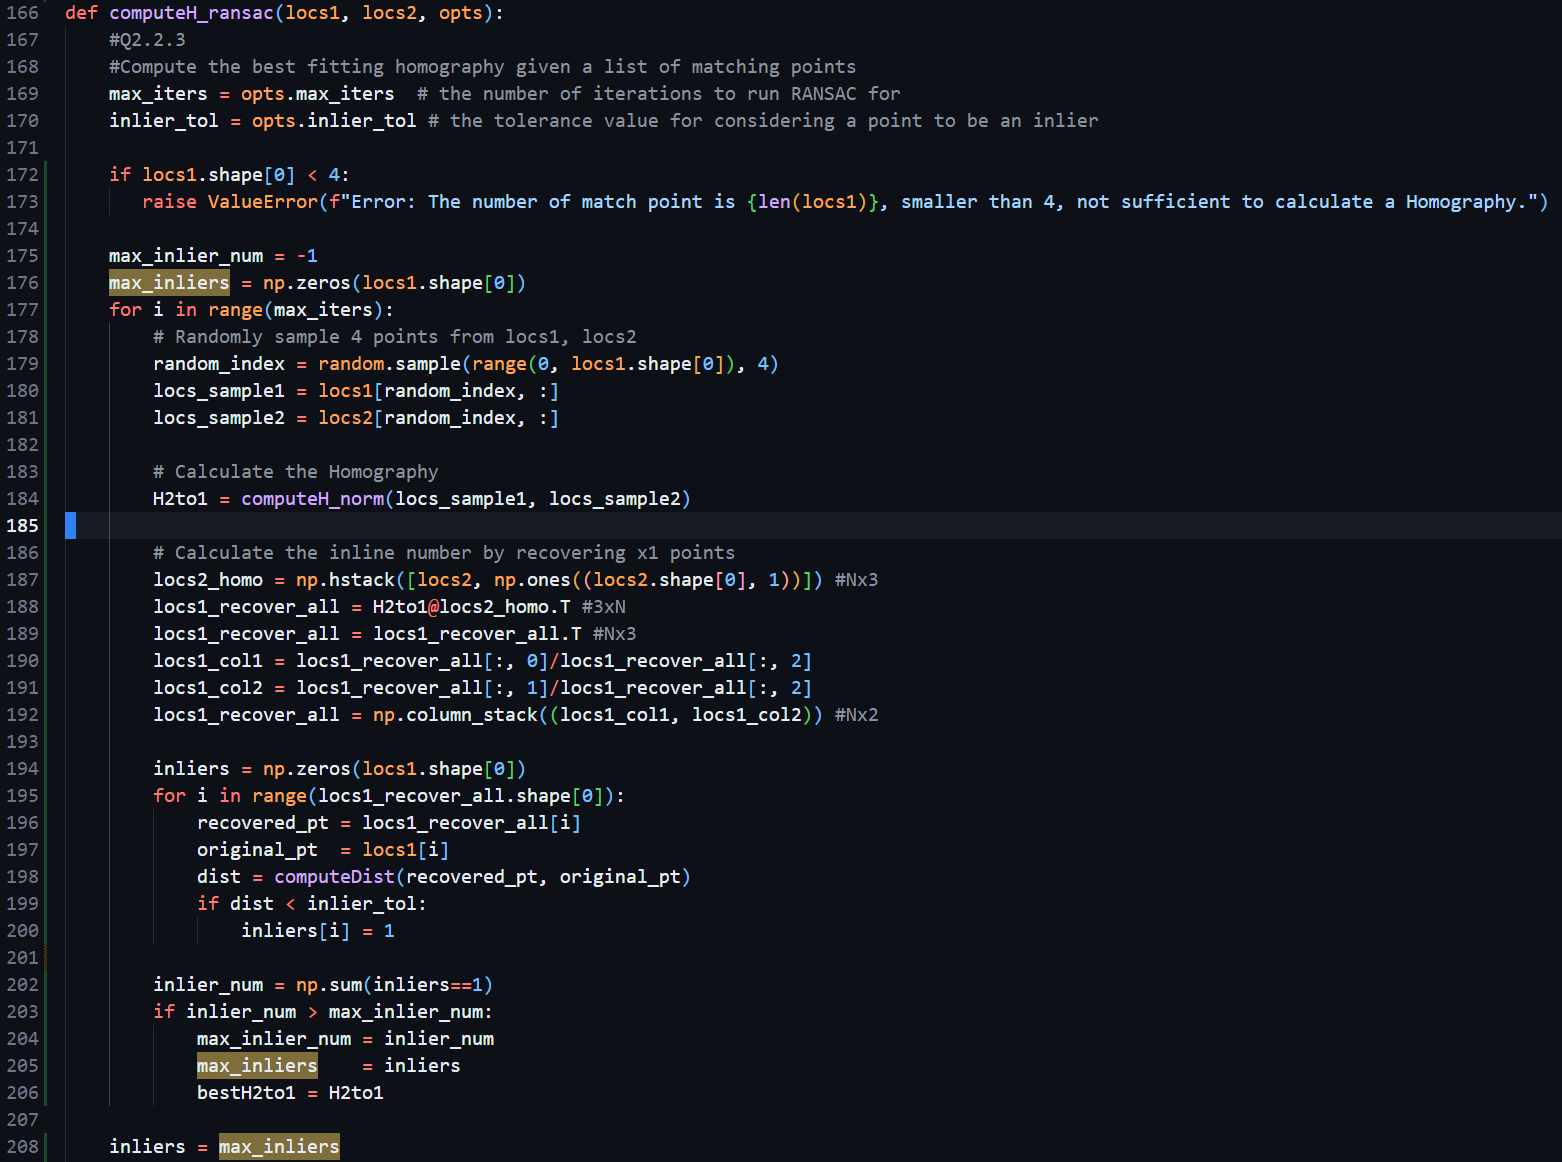
\includegraphics[width=\textwidth]{Q2_2_3_cns1.png}  % Replace with your image file
		\caption{Q2.2.3 Code Snippet 1}
		\label{fig:Q223_cns1}
	\end{minipage}
	\hfill  % This adds space between the images
	\begin{minipage}[b]{0.45\textwidth}
		\centering
		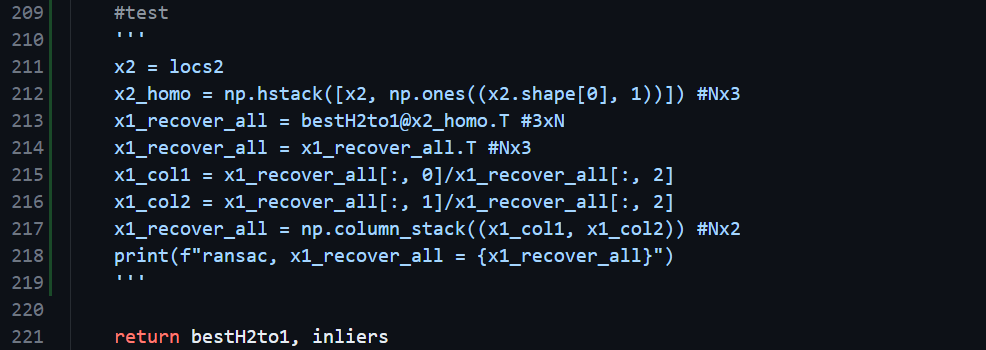
\includegraphics[width=\textwidth]{Q2_2_3_cns2.png}  % Replace with your image file
		\caption{Q2.2.3. Code Snippet 2}
		\label{fig:Q223_csn2}
	\end{minipage}	
	\end{figure}
	
	\newpage
	\subsection*{Q2.2.4 at page 8}
	Ans:\\
	\hangindent=0.4em \hspace{0.3em} Figure \ref{fig:Q224_result} shows the result image, and Figure \ref{fig:Q224_warpImage_cns} - Figure \ref{fig:Q224_compositeH_cns} show the code snippet. Besides, in the step4, the reason that the book space in cv\_desk.png is not filled up is that the size of hp\_cover.jpg is not the same as cv\_cover.jpg, and the homography warping cause some blank pixels without any mapping intensity values.
	The solution is to resize the hp\_cover.jpg to the size of cv\_cover.jpg as shown in Figure \ref{fig:Q224_warpImage_cns} line 32.
	\begin{figure}[H]		
	\centering
	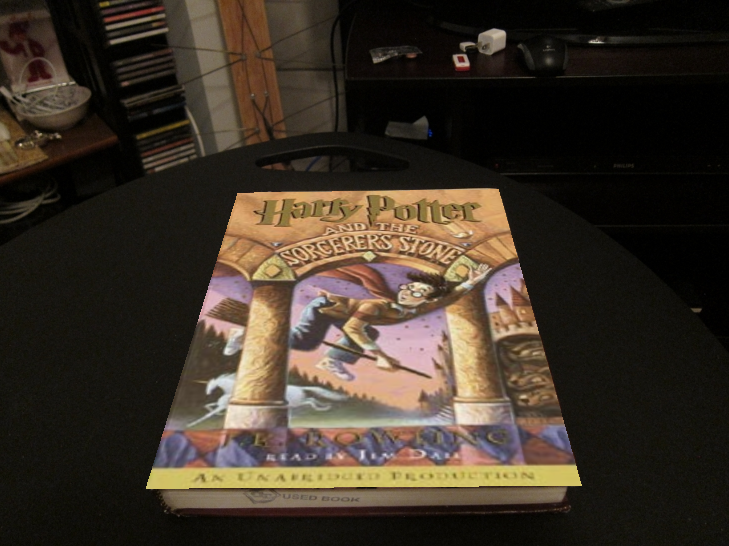
\includegraphics[width=0.8\textwidth]{Q2_2_4_result.png}  % Replace with your image file name
	\caption{Q2.2.4 Result Image}
	\label{fig:Q224_result}
	\end{figure}	
	\begin{figure}[H]
	\centering
	\begin{minipage}[b]{0.45\textwidth}
		\centering
		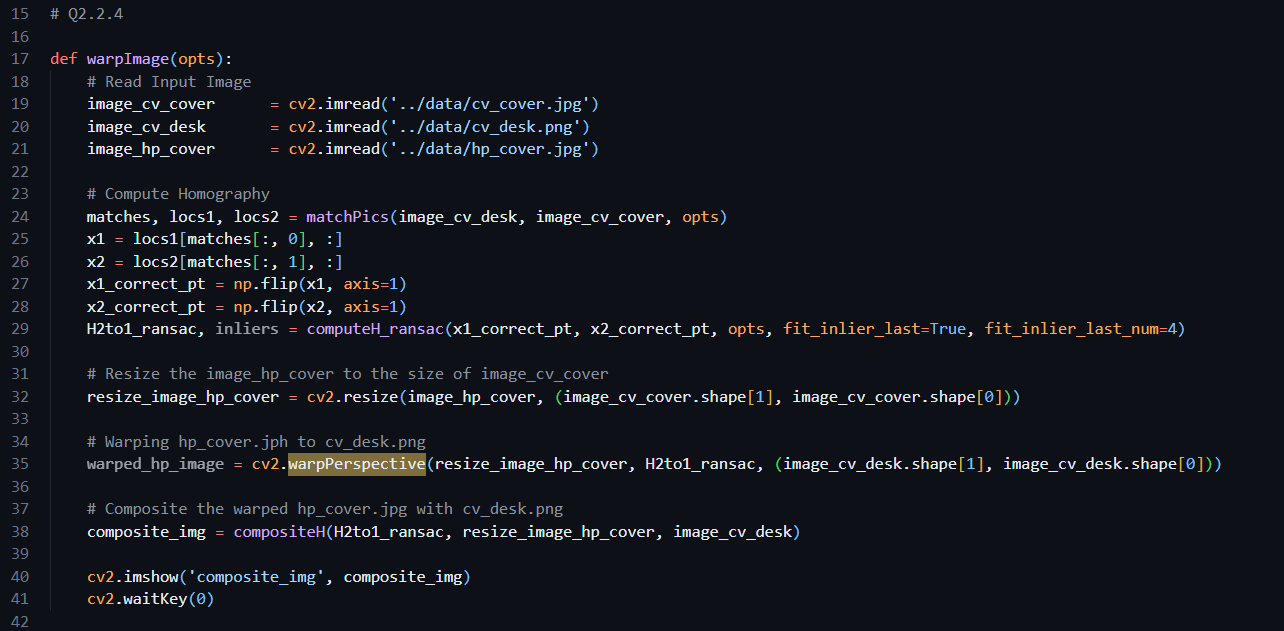
\includegraphics[width=\textwidth]{Q2_2_4_warpImage_cns.png}  % Replace with your image file
		\caption{Q2.2.4 warpImage() Code Snippet}
		\label{fig:Q224_warpImage_cns}
	\end{minipage}
	\hfill  % This adds space between the images
	\begin{minipage}[b]{0.45\textwidth}
		\centering
		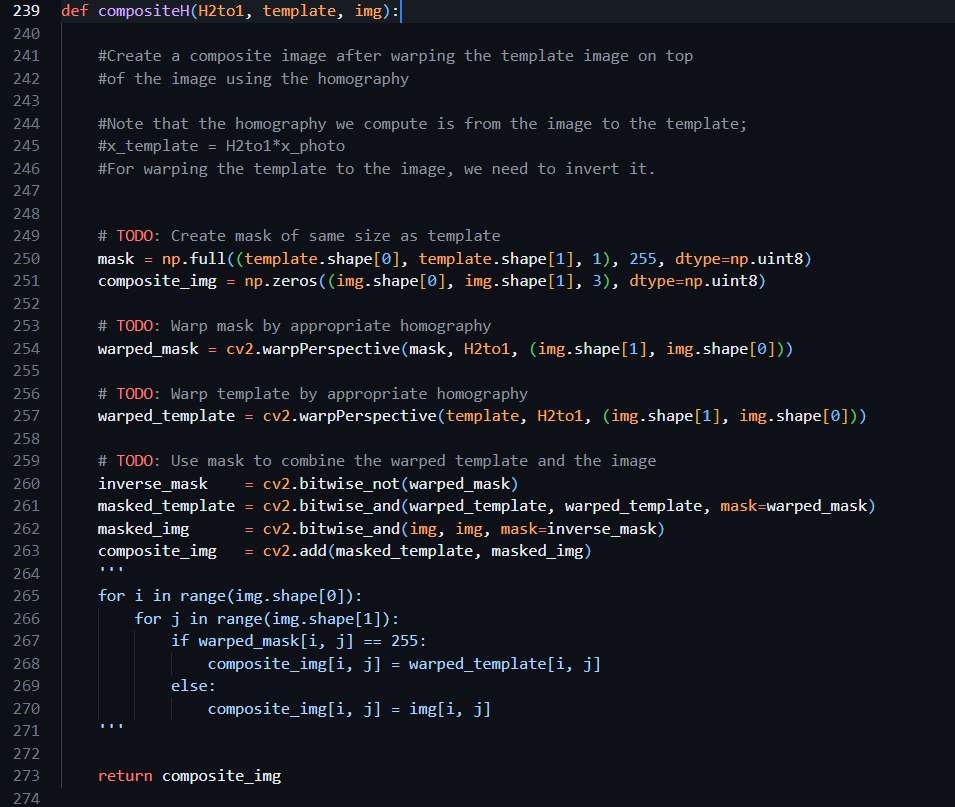
\includegraphics[width=\textwidth]{Q2_2_4_compositH_cns.png}  % Replace with your image file
		\caption{Q2.2.4. CompositeH() Code Snippet}
		\label{fig:Q224_compositeH_cns}
	\end{minipage}	
	\end{figure}	
	
	\newpage
	\subsection*{Q2.2.5 at page 8}
	Ans:\\
	\hangindent=0.4em \hspace{0.3em} Table \ref{table:composite} shows the result of different setting among parameters 'max\_iters' and 'inlier\_tol'. According to equation (22) specified in the slides of lecture, as the inlier\_tol decreases, it makes the feature points harder to be considered as an inlier, so the inlier rate w would decrease, and it makes the k (max\_iters), the number of trials that can gaurantee a return of a good model, increased too. On the opposite, if inlier\_tol increases, w would increase, and thus k (max\_iters) would decrease. However, in Table \ref{table:composite}, $2^{nd}$ row increase the inlier\_tol from 2.0 to 10.0, and the result seems not quite good. The reason is that at the end of computeH\_ransac() function, I would use all inliers again to fit an optimized homography. If the inlier\_tol is too large, then some outlier match points may be deemed as inlier, and they would be included into the last step calculating of optimized homography, making the result worse. On the other hand, from $4^{th}$ row to $5^{th}$ row, the inlier\_tol is decreased from 1 to 0.001, and the result seems worse in a great amount. The reason is that when iter\_tol is too low, then most of the time the homography is calculated using outliers. Sometimes the homography is truly computed by true inliers, but the number of inlier just equals to those fitting using outliers because of the very low value of iter\_tol. Accordingly, the RANSAC model selection process through inliers would become ineffective. In this problem,  according to my experiments, the appropriate range for inlier\_tol should be [0.5, 8], and the max\_iters set to 500 is enough.
	\begin{equation}
	k = \frac{\log(1 - p)}{\log(1 - w^n)}
	\end{equation}	
	\begin{table}[H]
	\centering
	\begin{tabular}{|c|c|c|}
		\hline
		\textbf{Parameter max\_iters} & \textbf{Parameter inlier\_tol} & \textbf{Composite Image} \\
		\hline
		500 & 2.0 & 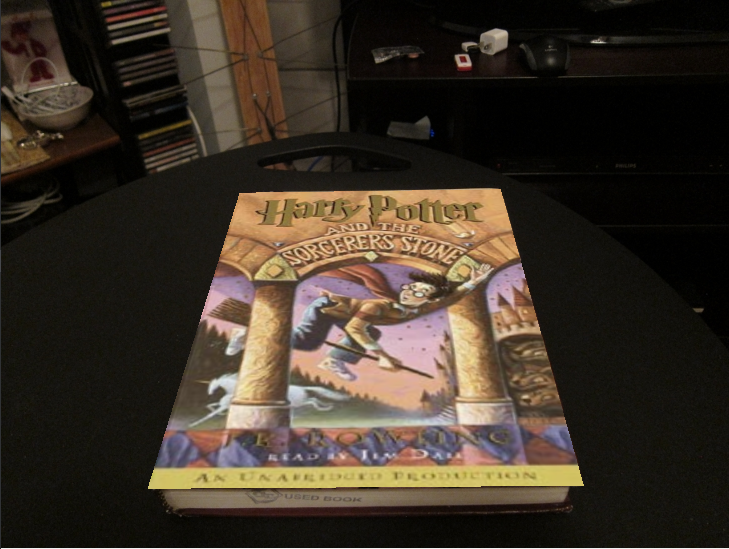
\includegraphics[width=0.27\textwidth]{Q2_2_5_500_2.0.png} \\
		\hline
		500 & 10.0 & 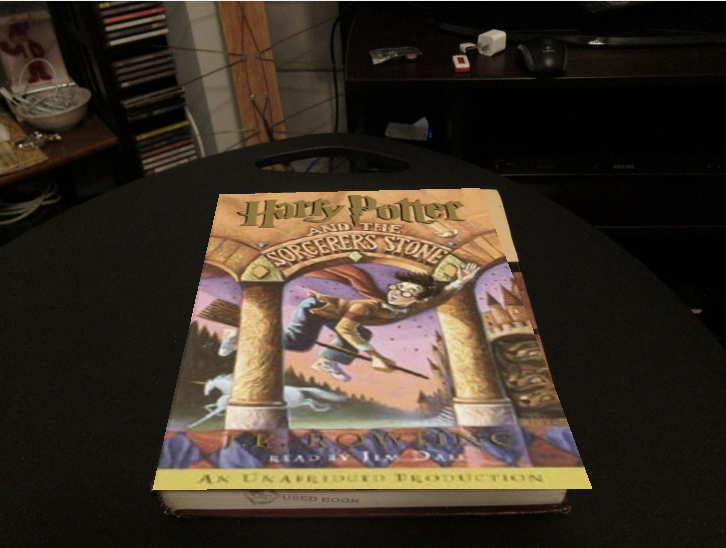
\includegraphics[width=0.27\textwidth]{Q2_2_5_500_10.0.png} \\						
		\hline
		5000 & 2.0 & 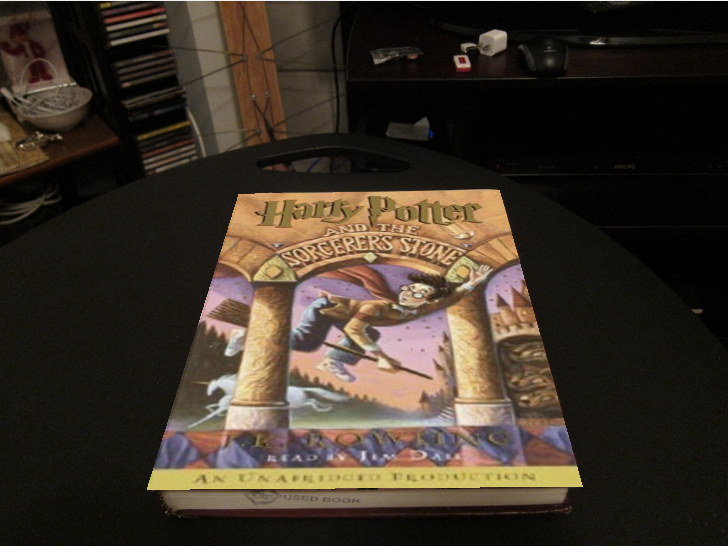
\includegraphics[width=0.27\textwidth]{Q2_2_5_5000_2.0.png} \\
		\hline
		500 & 1.0 & 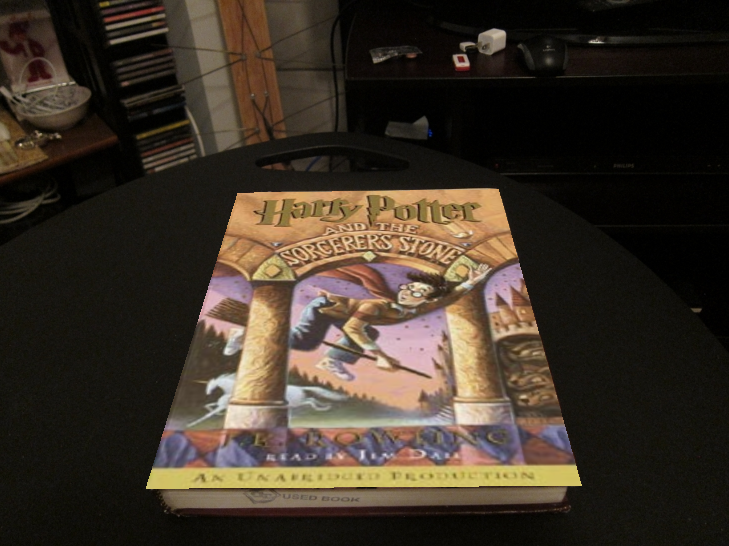
\includegraphics[width=0.27\textwidth]{Q2_2_5_500_1.0.png} \\			
		\hline
		500 & 0.001 & 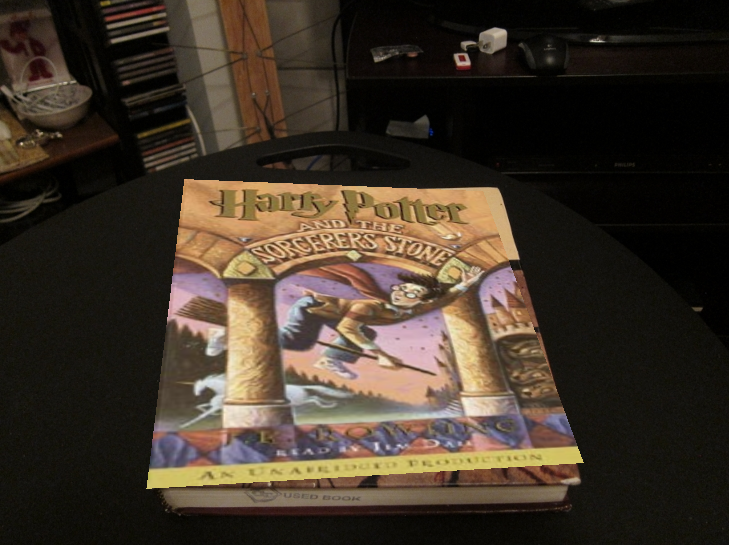
\includegraphics[width=0.27\textwidth]{Q2_2_5_500_0.001.png} \\
		\hline
		5000 & 0.001 & 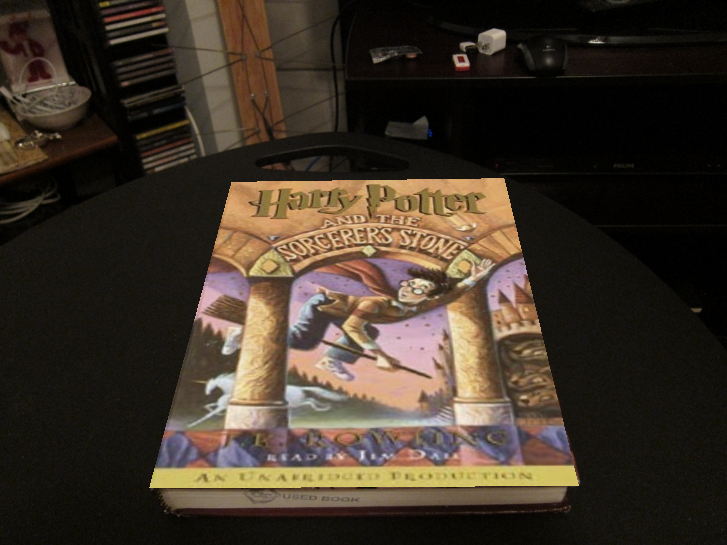
\includegraphics[width=0.27\textwidth]{Q2_2_5_5000_0.001.png} \\
		\hline
	\end{tabular}
	\caption{Parameter Changes and Corresponding Composite Images}
	\label{table:composite}
	\end{table}	
	
	\newpage
	\subsection*{Q3.1 at page 9}
	Ans:\\
	\hangindent=0.4em \hspace{0.3em} Figure \ref{fig:Q331_left} - Figure \ref{fig:Q331_cnter} shows the results of composite video where the timestamps displaying overlays at left, right, and center of the video frame. The resulted video is here: \href{https://drive.google.com/file/d/1lg2Ez4O62NCa-MrrvyQUnXDzLBnftsAt/view?usp=sharing}{ar\@.avi}, and the code snippets are as the following Figure \ref{fig:Q331_cns1} - Figure \ref{fig:Q331_cns3}.
	\begin{figure}[H]
	\centering
	\begin{minipage}[b]{0.45\textwidth}
		\centering
		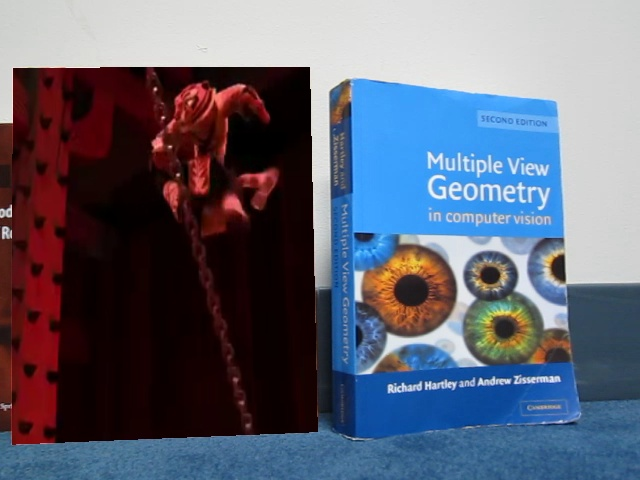
\includegraphics[width=\textwidth]{./result/Q3_1_ar_result_overlay_left.jpg}  % Replace with your image file
		\caption{Q3.1 Screenshot of Result at Left Timestamp}
		\label{fig:Q331_left}
	\end{minipage}
	\hfill  % This adds space between the images
	\begin{minipage}[b]{0.45\textwidth}
		\centering
		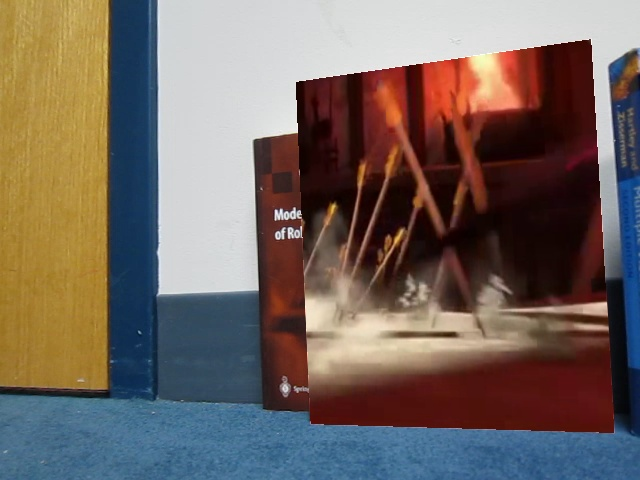
\includegraphics[width=\textwidth]{./result/Q3_1_ar_result_overlay_right.jpg}  % Replace with your image file
		\caption{Q3.1 Screenshot of Result at Right Timestamp}
		\label{fig:Q331_right}
	\end{minipage}
	\end{figure}	
	
	\begin{figure}[H]		
	\centering
	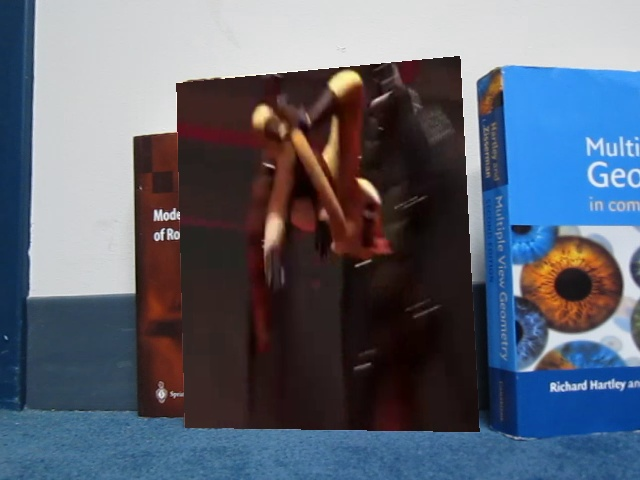
\includegraphics[width=0.45\textwidth]{./result/Q3_1_ar_result_overlay_cnter.jpg}  % Replace with your image file
	\caption{Q3.1 Screenshot of Result at Center Timestamp}
	\label{fig:Q331_cnter}
	\end{figure}	
	
	\begin{figure}[H]
	\centering
	\begin{minipage}[b]{0.45\textwidth}
		\centering
		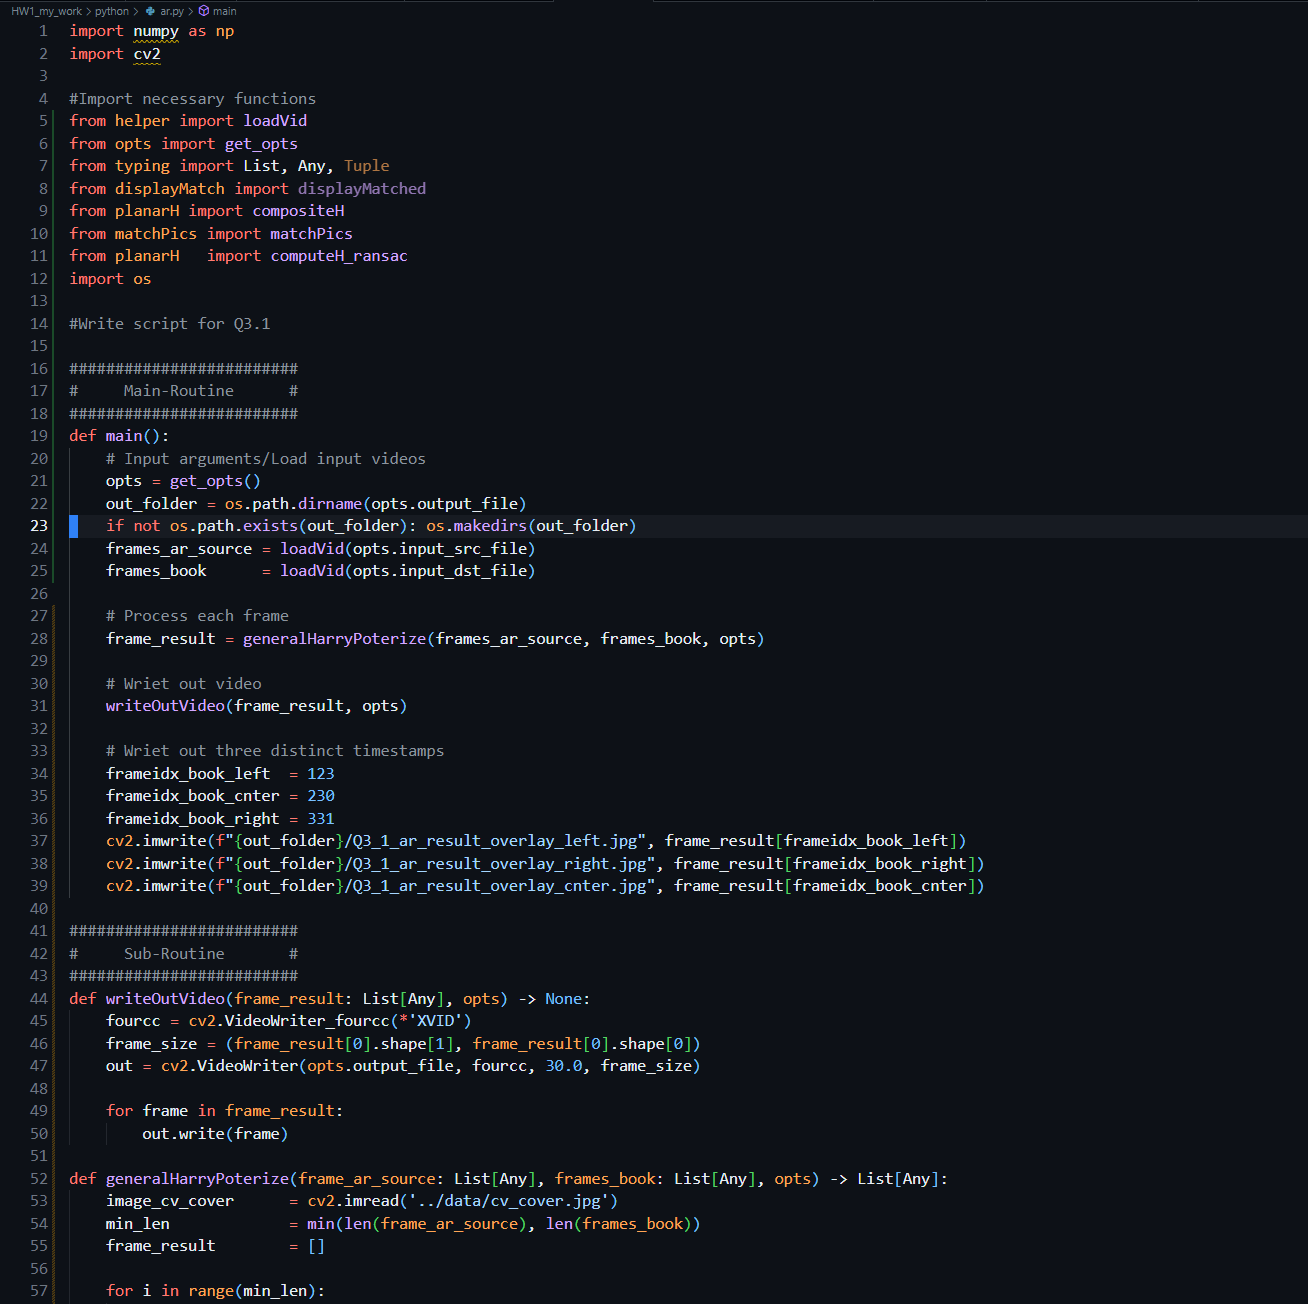
\includegraphics[width=\textwidth]{./Q3_1_ar_cns1.png}  % Replace with your image file
		\caption{Q3.1 Code Snippet 1}
		\label{fig:Q331_cns1}
	\end{minipage}
	\hfill  % This adds space between the images
	\begin{minipage}[b]{0.45\textwidth}
		\centering
		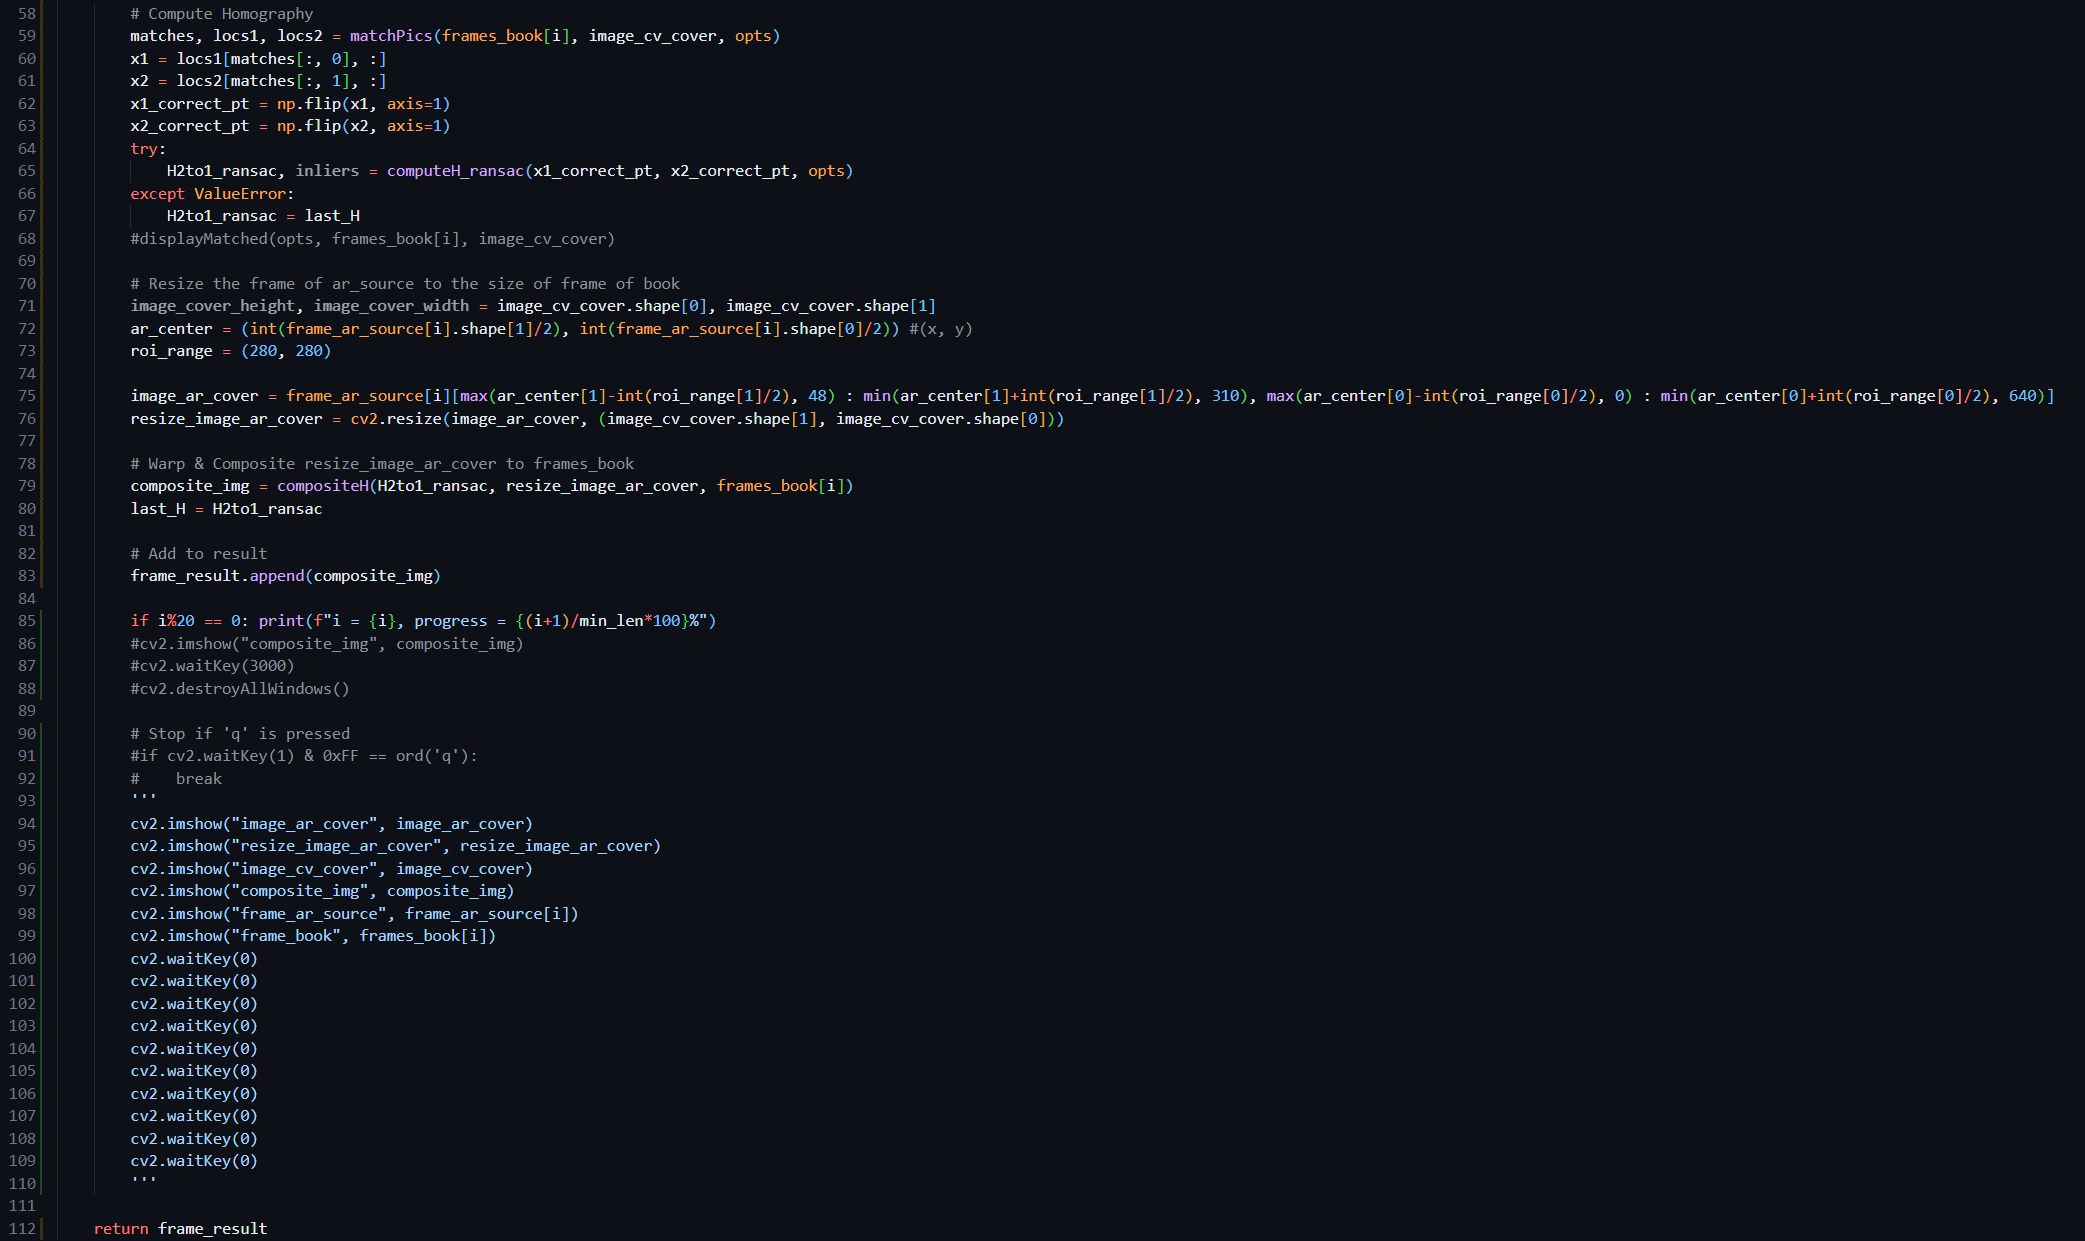
\includegraphics[width=\textwidth]{./Q3_1_ar_cns2.png}  % Replace with your image file
		\caption{Q3.1 Code Snippet 2}
		\label{fig:Q331_cns2}
	\end{minipage}
	\end{figure}
	\begin{figure}[H]		
	\centering
	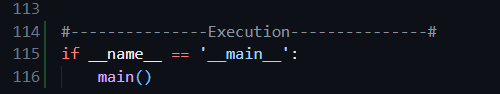
\includegraphics[width=0.45\textwidth]{./Q3_1_ar_cns3.png}  % Replace with your image file
	\caption{Q3.1 Code Snippet 3}
	\label{fig:Q331_cns3}
	\end{figure}		
	
	\newpage
	\subsection*{Q3.2 at page 10}
	Ans:\\
	\hangindent=0.4em \hspace{0.3em} In order to accelerate the whole program to approach the real-time performance, I firstly need to know which part of the program takes long time to process. To get the 30 FPS result, each for loop to process a frame should use less than 1/30 seconds, nearly 0.03 seconds. Figure \ref{fig:Q32profiling} shows the code I added to do the profiling, and Figure \ref{fig:Q32profiling_result} shows the result. As we can see from the result, both the time used to compute BRIEF descriptor and the match of the BRIEF descriptors take longer than 0.03 seconds, that is, original BRIEF descriptor takes 7.23 seconds to complete, and BRIEF matching takes 0.341 seconds to complete. One can reproduce the profiling result by referring to the command specified in python/README.md. When it comes to improving the whole process, my first thought is to down-sample the input frame, and use the smaller images (frames) to calculate feature detection, description, and matching, and then calculate the corresponding homography and rescale it to the original scale. The benefit is obvious: calculation on lower resolution reduces the processing time greatly. Hence, I did the following three changes:
	\begin{enumerate}
	\item Include a down\_sample\_factor input argument to specify the factor of down-sampling. Down-sample each of the frames before calculating feature detection, descriptor, matching, and homography. After calculating the homography, rescale it back to the original scale.
	\item Since I have the change of scaling, and the original implementation of FAST detector and BRIEF descriptor are not scale-invariant, I choose to replace them with Opencv built-in ORB detector and descriptor, which has both scale-invariance and rotation-invariance.
	\item As I have changed to the ORB detector and descriptor, the matching method should also be changed. According to \href{https://stackoverflow.com/questions/10610966/difference-between-bfmatcher-and-flannbasedmatcher}{this discussion} and \href{https://docs.opencv.org/4.x/dc/dc3/tutorial_py_matcher.html}{OpenCV website}, I would choose FLANN based Matcher over BFMatcher.
	\end{enumerate}
	\begin{figure}[H]
		\centering
		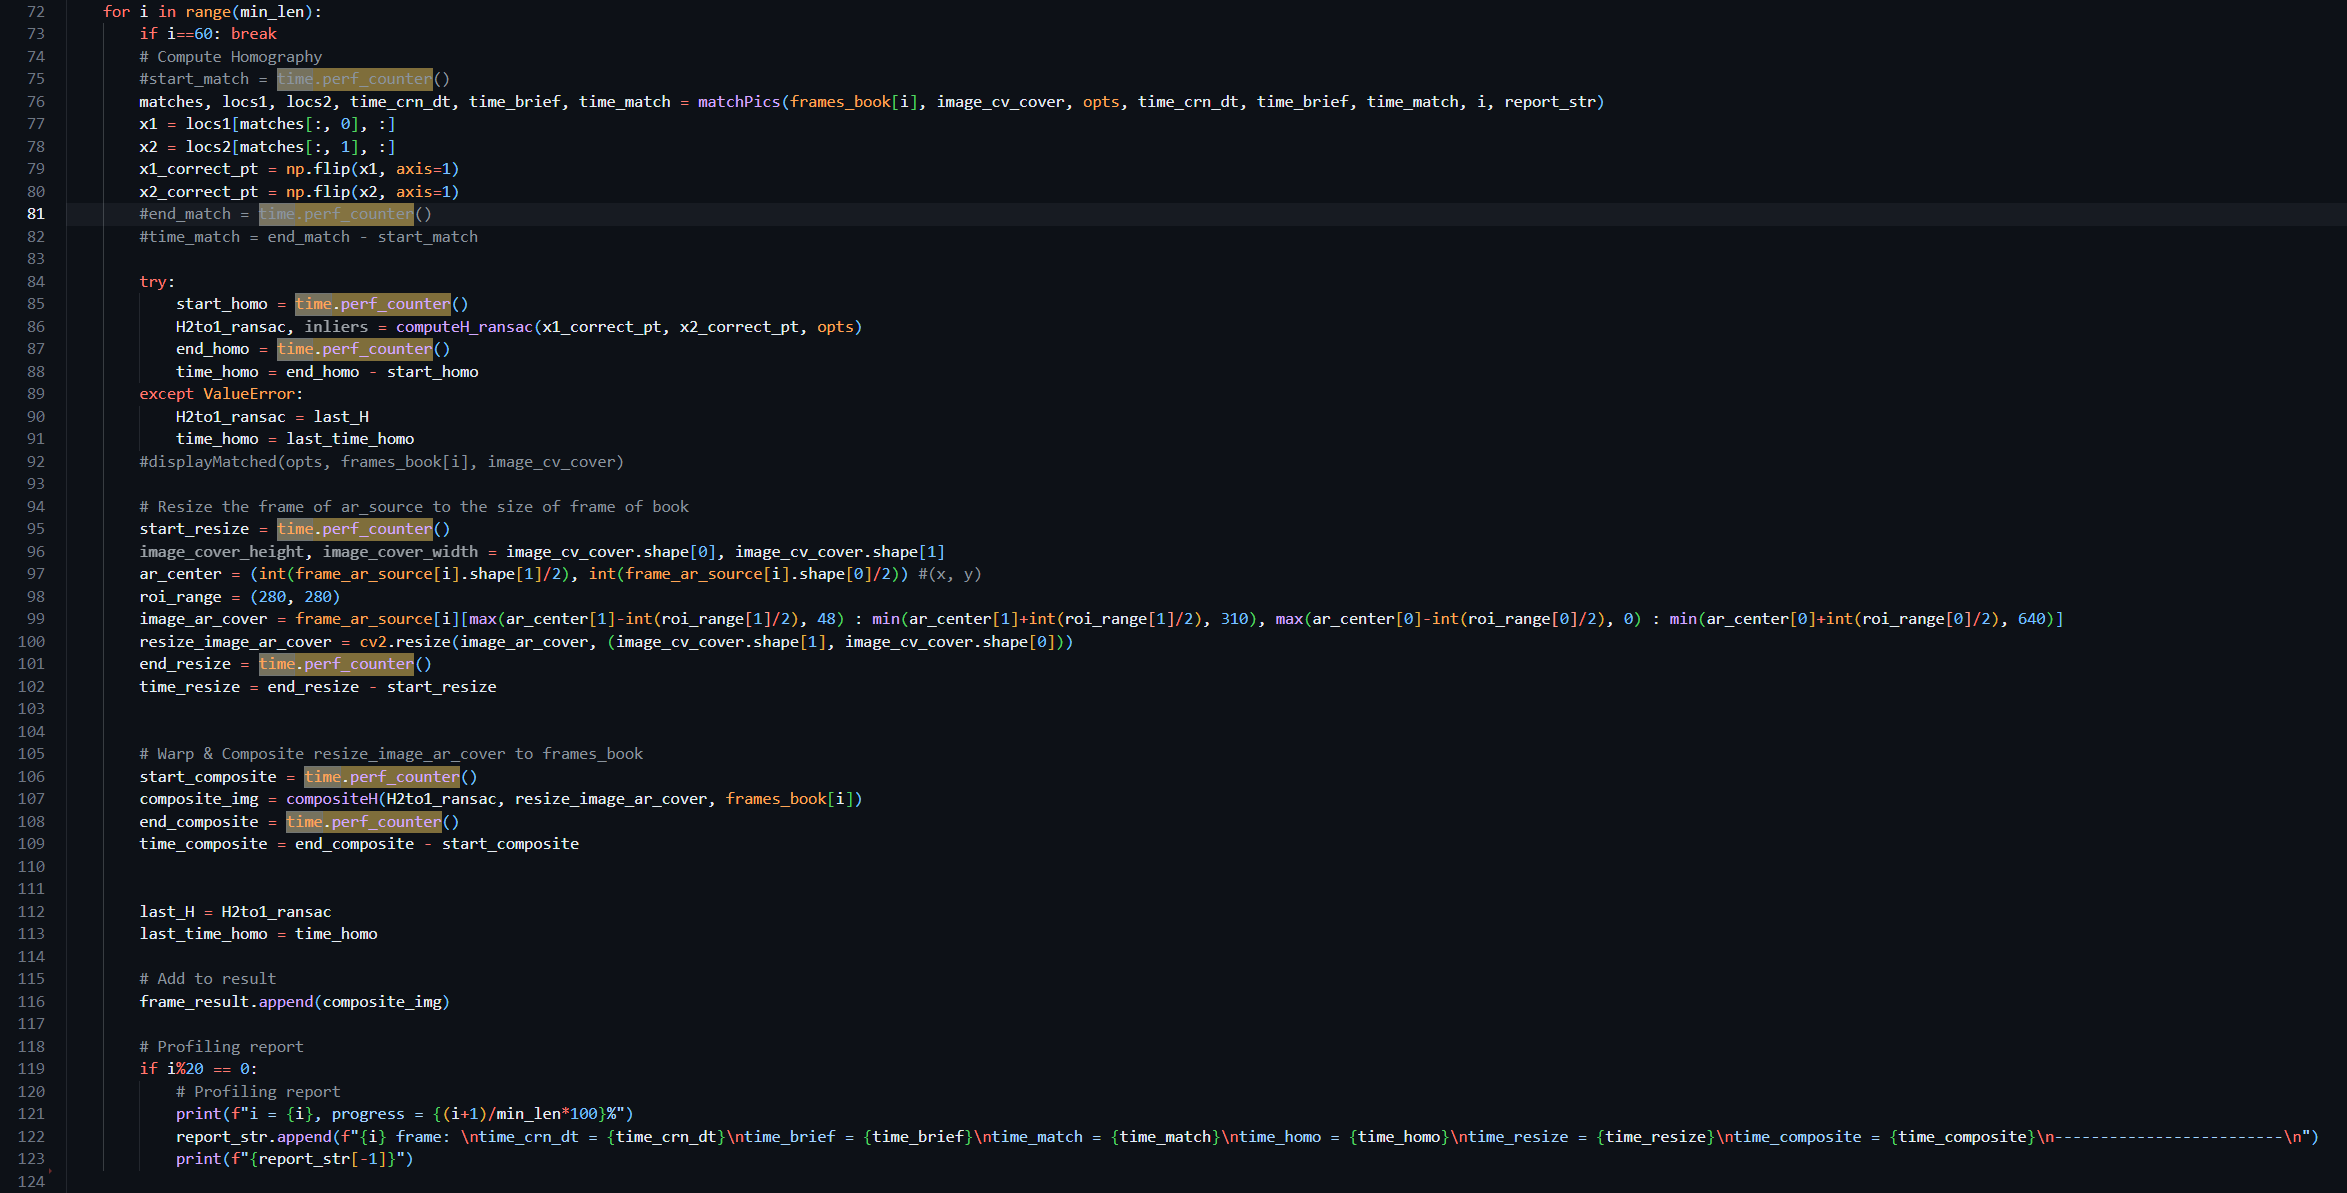
\includegraphics[width=0.7\textwidth]{./Q3_2_ar_ec_profiling_cns1.png}  % Replace with your image file
		\caption{Q3.2 Profiling Code Snippet}
		\label{fig:Q32profiling}
	\end{figure}	
	\begin{figure}[H]
		\centering
		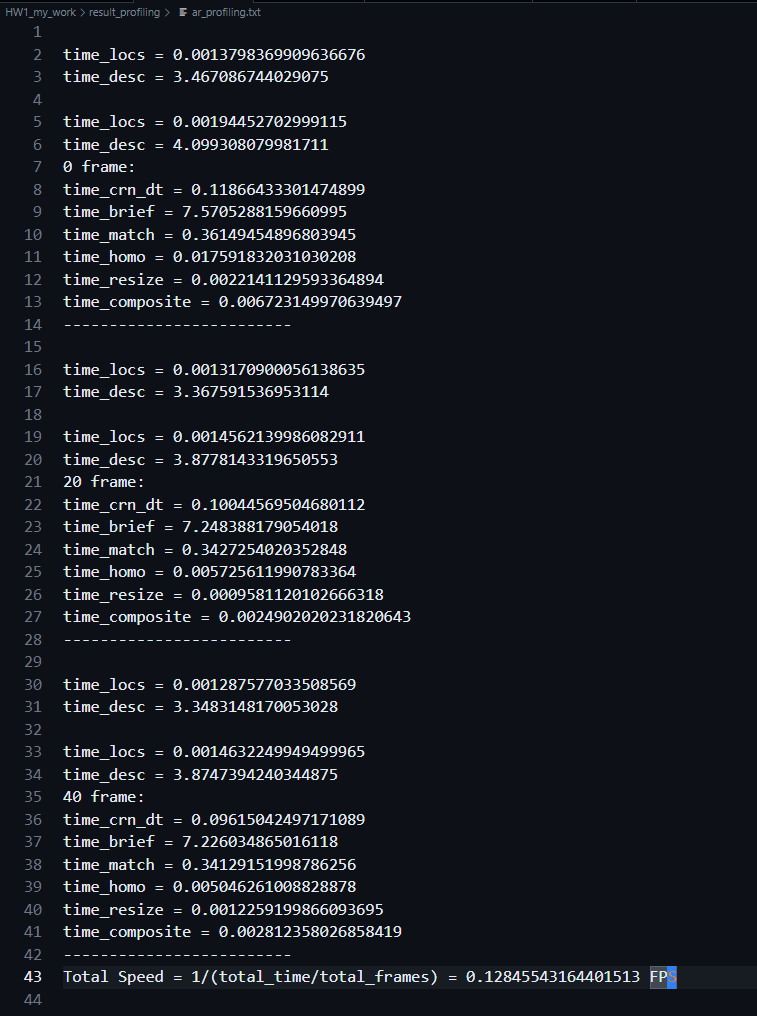
\includegraphics[width=0.5\textwidth]{./Q3_2_ar_ec_profiling_result.png}  % Replace with your image file
		\caption{Q3.2 Profiling Result}
		\label{fig:Q32profiling_result}
	\end{figure}	
	\hangindent=0.1em \hspace{0.1em}Figure \ref{fig:Q32_change1_cns1} shows the code snippet of change 1 occuring in ec/matchPics.py matchPics(), which I down-sample the two gray images before calculating the feature points. Figure \ref{fig:Q32_change1_cns2} shows the code snippet of change 1 occuring in ec/planarH.py computeH\_ransac(), which I scale back the calculated homography to the original scale by multiplying the down\_sample\_factor on the translation part of the homography, and leaves other parts unchanged as other parts do not change due to down-sampling.


	\begin{figure}[H]
	\centering
	\begin{minipage}[b]{0.45\textwidth}
		\centering
		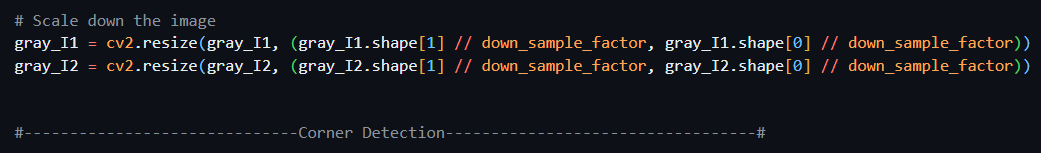
\includegraphics[width=\textwidth]{./Q3_2_ar_ec_change1_cns1.png}  % Replace with your image file
		\caption{Q3.2 Change 1 Code Snippet 1}
		\label{fig:Q32_change1_cns1}
	\end{minipage}
	\hfill  % This adds space between the images
	\begin{minipage}[b]{0.45\textwidth}
		\centering
		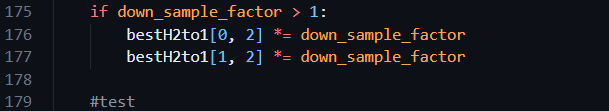
\includegraphics[width=\textwidth]{./Q3_2_ar_ec_change1_cns2.png}  % Replace with your image file
		\caption{Q3.2 Change 1 Code Snippet 2}
		\label{fig:Q32_change1_cns2}
	\end{minipage}
	\end{figure}
	\hangindent=0.1em \hspace{0.1em}Figure \ref{fig:Q32_change2_cns1} shows the change 2 occuring in ec/matchPics.py matchPics(), where I call the Opencv built-in ORB function to find the corresponding detectors and descriptors. 
		
	\begin{figure}[H]
		\centering
		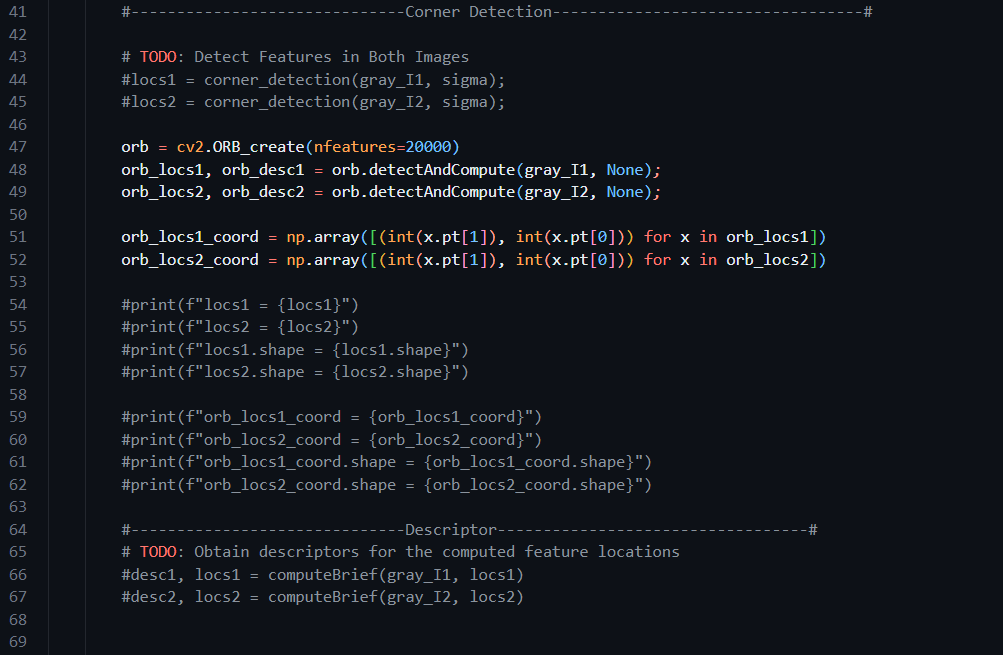
\includegraphics[width=0.7\textwidth]{./Q3_2_ar_ec_change2_cns1.png}  % Replace with your image file
		\caption{Q3.2 Change 2 Code Snippet}
		\label{fig:Q32_change2_cns1}
	\end{figure}
	\hangindent=0.1em \hspace{0.1em}Figure \ref{fig:Q32_change3_cns1} shows the change 3 occuring in ec/matchPics.py matchPics(), where I call the Opencv built-in ORB matching function, called FLANN based Matcher, to find the corresponding matching feature points.
	
	\begin{figure}[H]
	\centering
	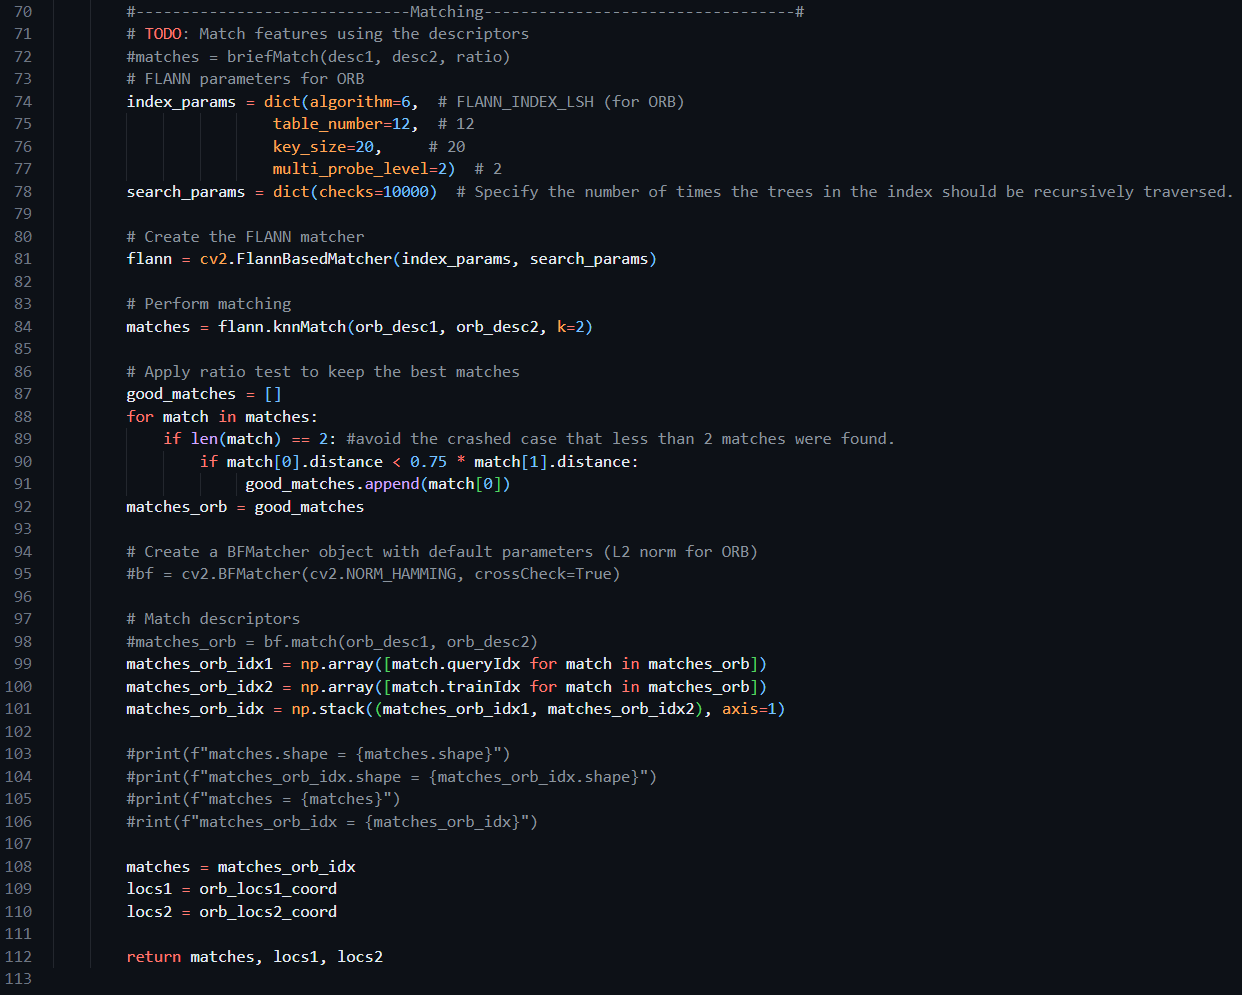
\includegraphics[width=0.7\textwidth]{./Q3_2_ar_ec_change3_cns1.png}  % Replace with your image file
	\caption{Q3.2 Change 3 Code Snippet}
	\label{fig:Q32_change3_cns1}
	\end{figure}
	
	\hangindent=0.1em \hspace{0.1em}Figure \ref{fig:Q32_ar_ec_cns1} - Figure \ref{fig:Q32_ar_ec_cns3} show the code snippet of the main function in ec/ar\_ec.py. One can refer to ec/README.md for the command to run the real-time AR application. The final FPS will be automatically reported on the standard output and the report willl be stored under the folder specified by --output\_file argument. The resulting video will also be stored in the same output folder. The final performance under my environment is nearly 31 FPS as shown in Figure \ref{fig:Q32_ar_ec_fs}, which is 242 times faster over the original implementation with 0.128 FPS shown in Figure \ref{fig:Q32profiling_result}.
	
	\begin{figure}[H]
		\centering
		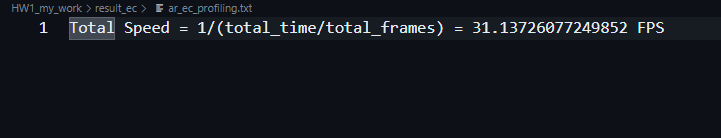
\includegraphics[width=0.7\textwidth]{./Q3_2_ar_ec_final_speed.png}  % Replace with your image file
		\caption{Q3.2 ar\_ec.py Final Speed}
		\label{fig:Q32_ar_ec_fs}
	\end{figure}	
	
	\begin{figure}[H]
		\centering
		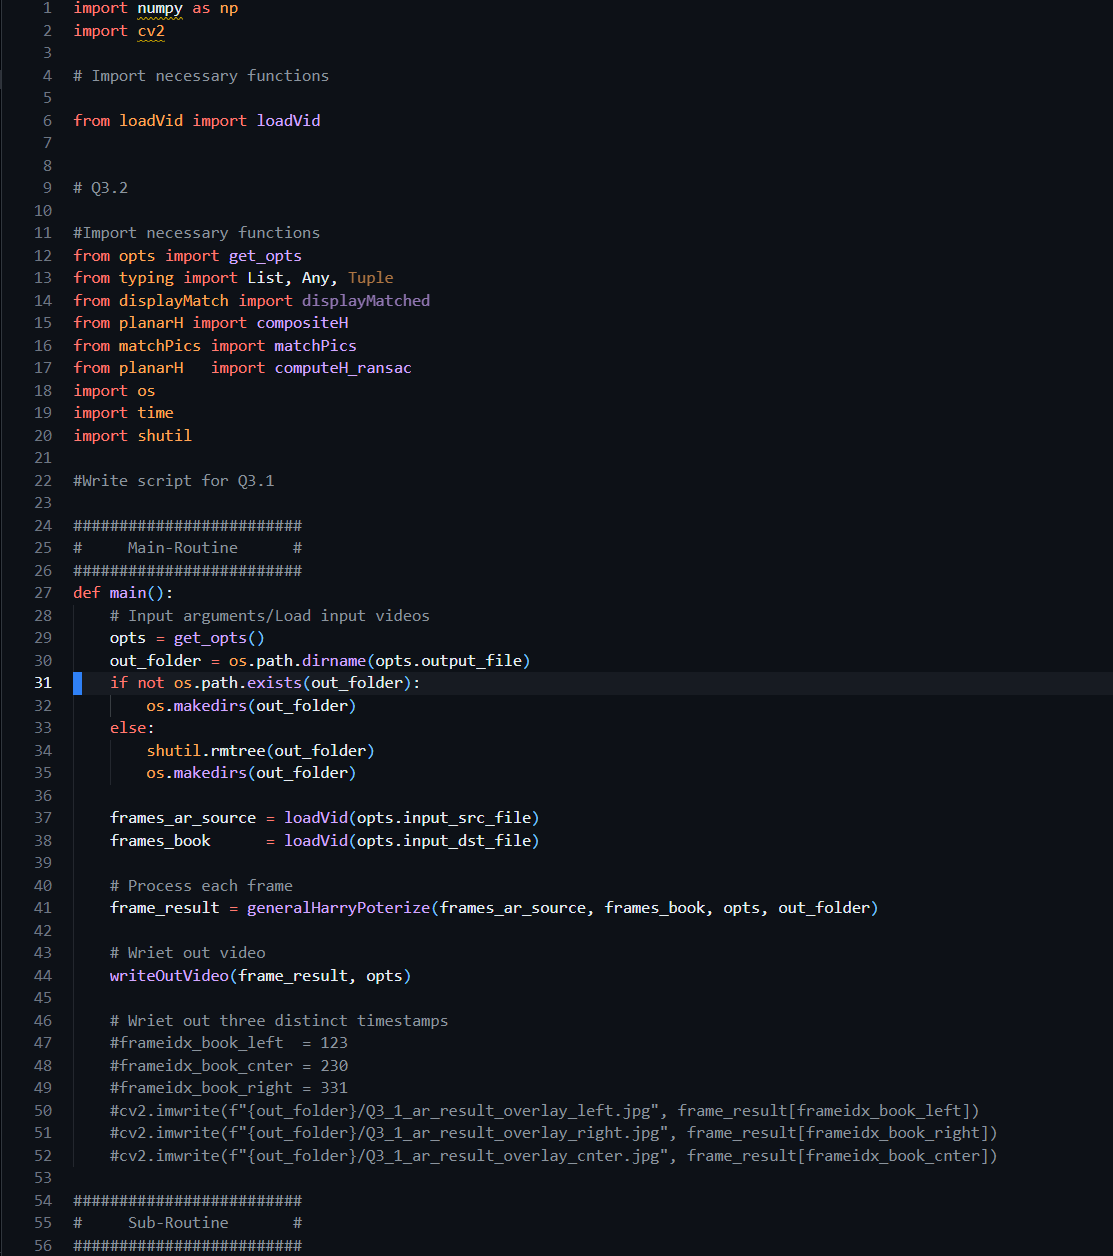
\includegraphics[width=0.7\textwidth]{./Q3_2_ar_ec_cns1.png}  % Replace with your image file
		\caption{Q3.2 ar\_ec.py Code Snippet 1}
		\label{fig:Q32_ar_ec_cns1}
	\end{figure}
	\begin{figure}[H]
		\centering
		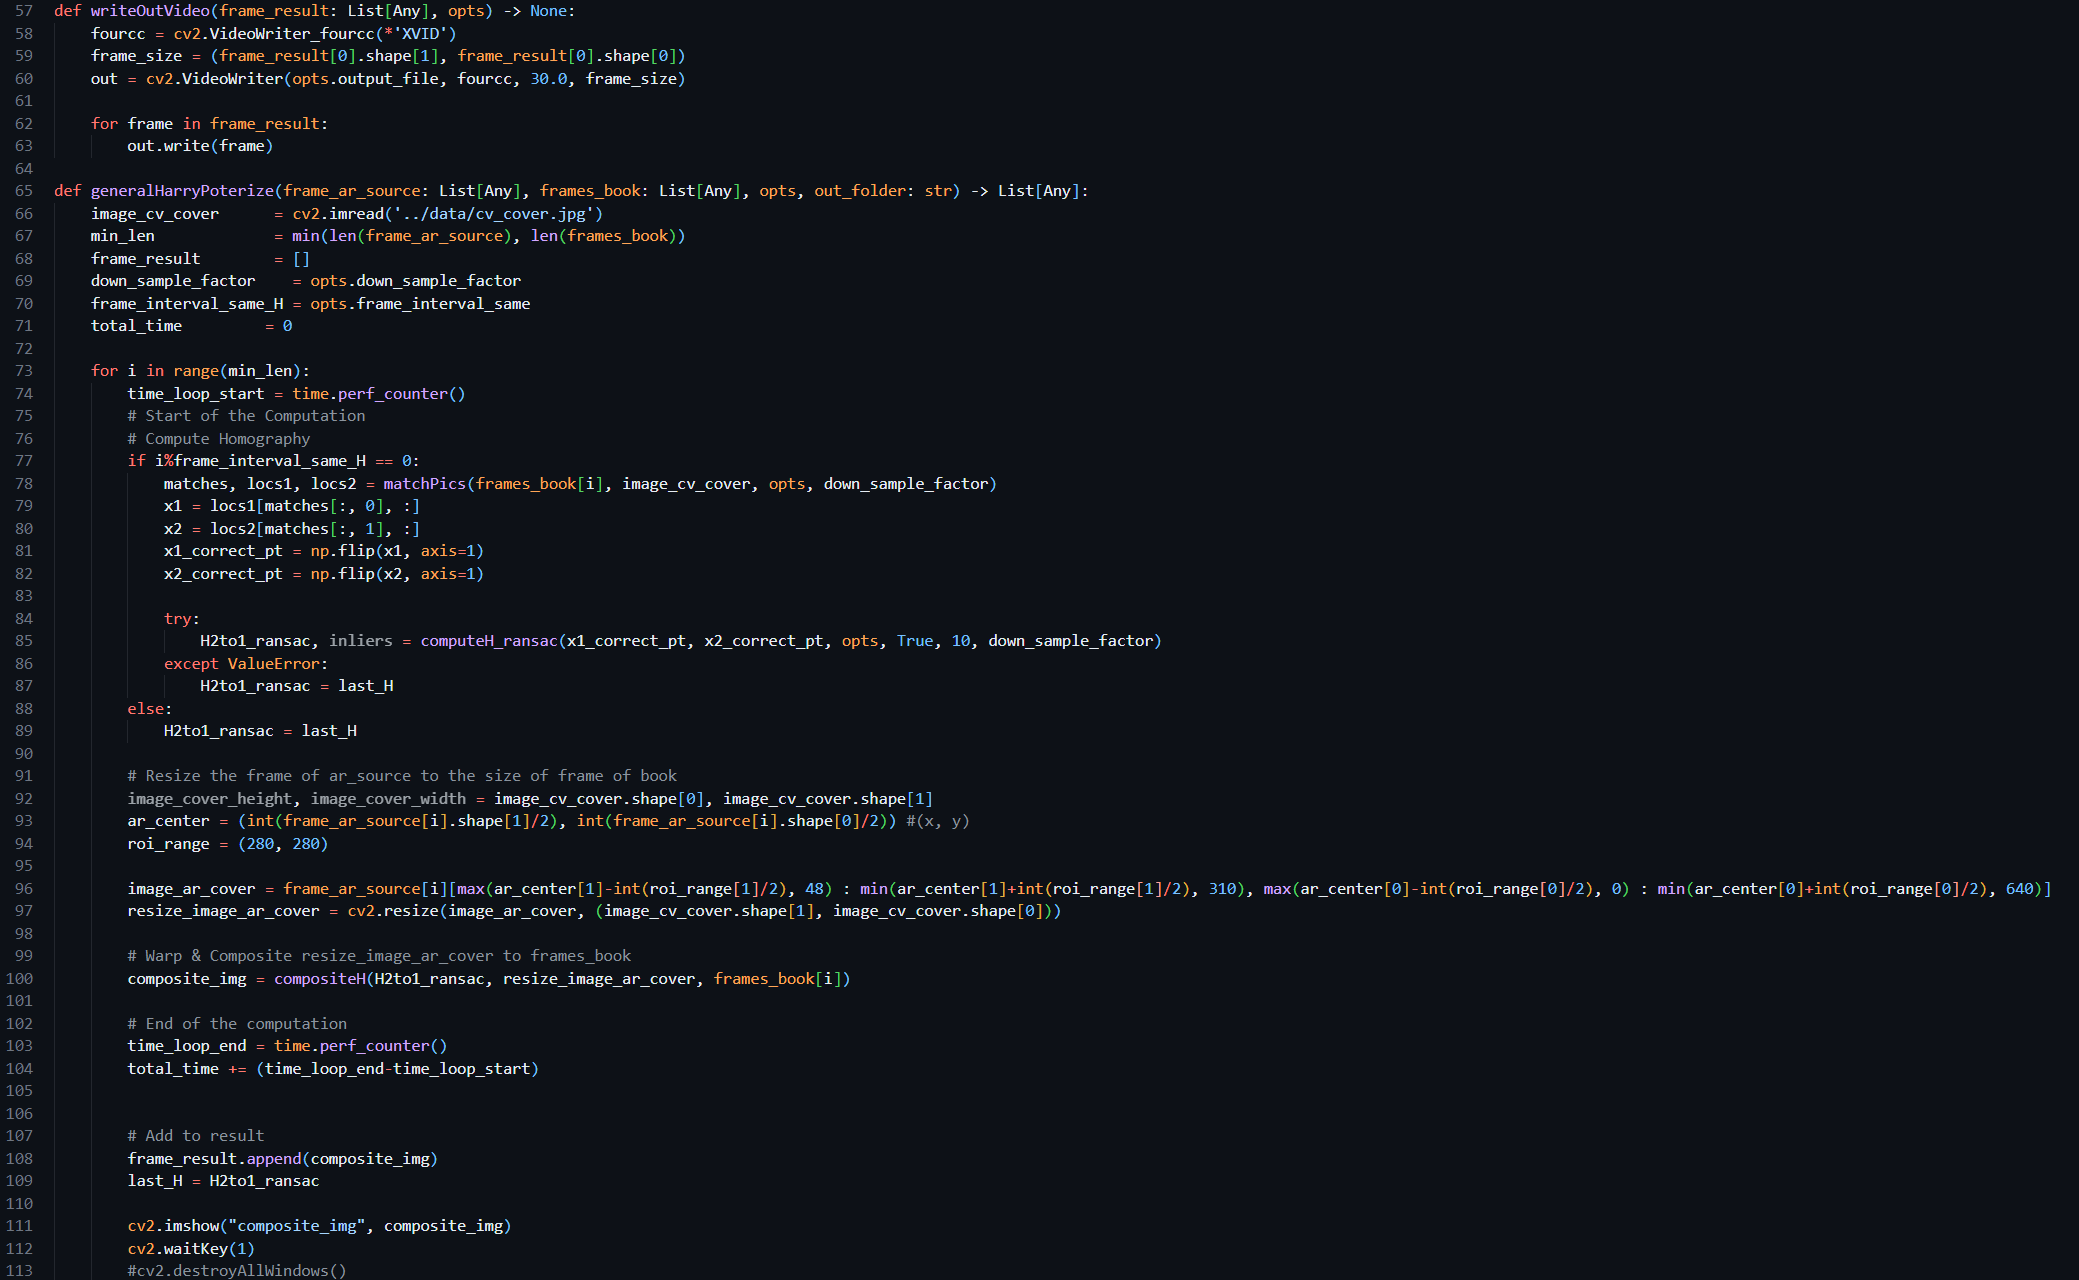
\includegraphics[width=\textwidth]{./Q3_2_ar_ec_cns2.png}  % Replace with your image file
		\caption{Q3.2 ar\_ec.py Code Snippet 2}
		\label{fig:Q32_ar_ec_cns2}
	\end{figure}
	\begin{figure}[H]
		\centering
		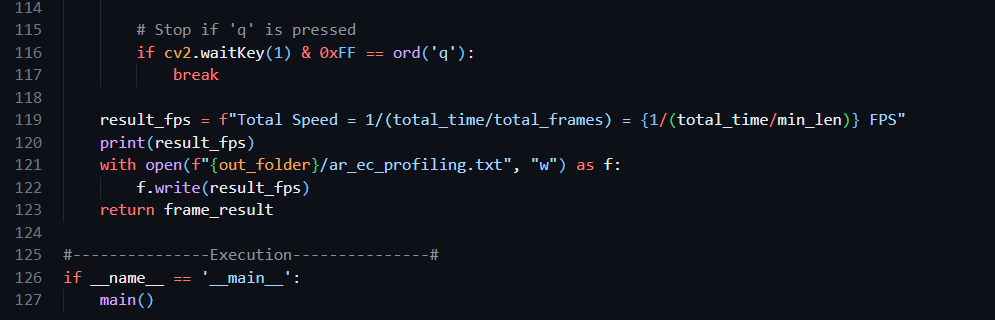
\includegraphics[width=\textwidth]{./Q3_2_ar_ec_cns3.png}  % Replace with your image file
		\caption{Q3.2 ar\_ec.py Code Snippet 3}
		\label{fig:Q32_ar_ec_cns3}
	\end{figure}
	\hangindent=0.1em \hspace{0.1em}There is another input argument that I originally developed to further speedup, but I currently do not use it. It is the --frame\_interval\_same. It is used to bypass some frames by using the same homography as previous frame. The reason that one can do it is to assume that the targeted frames will not have large movement over 'frame\_interval\_same' frames. Under this assumption, the mapping of homography can be deemed as nearly unchanged. The default value of this argument is set to 2 as I think that data/book.mov does not have big motion between continuous frames. Although I can use it to further speedup my performance, which may be up to 50 FPS, I do not turn it on by setting this argument to 1 , as the command specified in ec/README.md, because I have already reached the performance over 30 FPS without the usage of this argument.

	\newpage
	\subsection*{Q4 at page 10}
	Ans:\\
	\hangindent=0.4em \hspace{0.3em} Figure \ref{fig:Q4_input_left_img} shows my input left image, and Figure \ref{fig:Q4_input_right_img} shows my input right image, and Figure \ref{fig:Q4_result_pano} shows the result of generated panorama. Figure \ref{fig:Q4_cns1} - Figure \ref{fig:Q4_cns3} show my snippets of code that implement panorama.py.

	\begin{figure}[H]
	\centering
	\begin{minipage}[b]{0.45\textwidth}
		\centering
		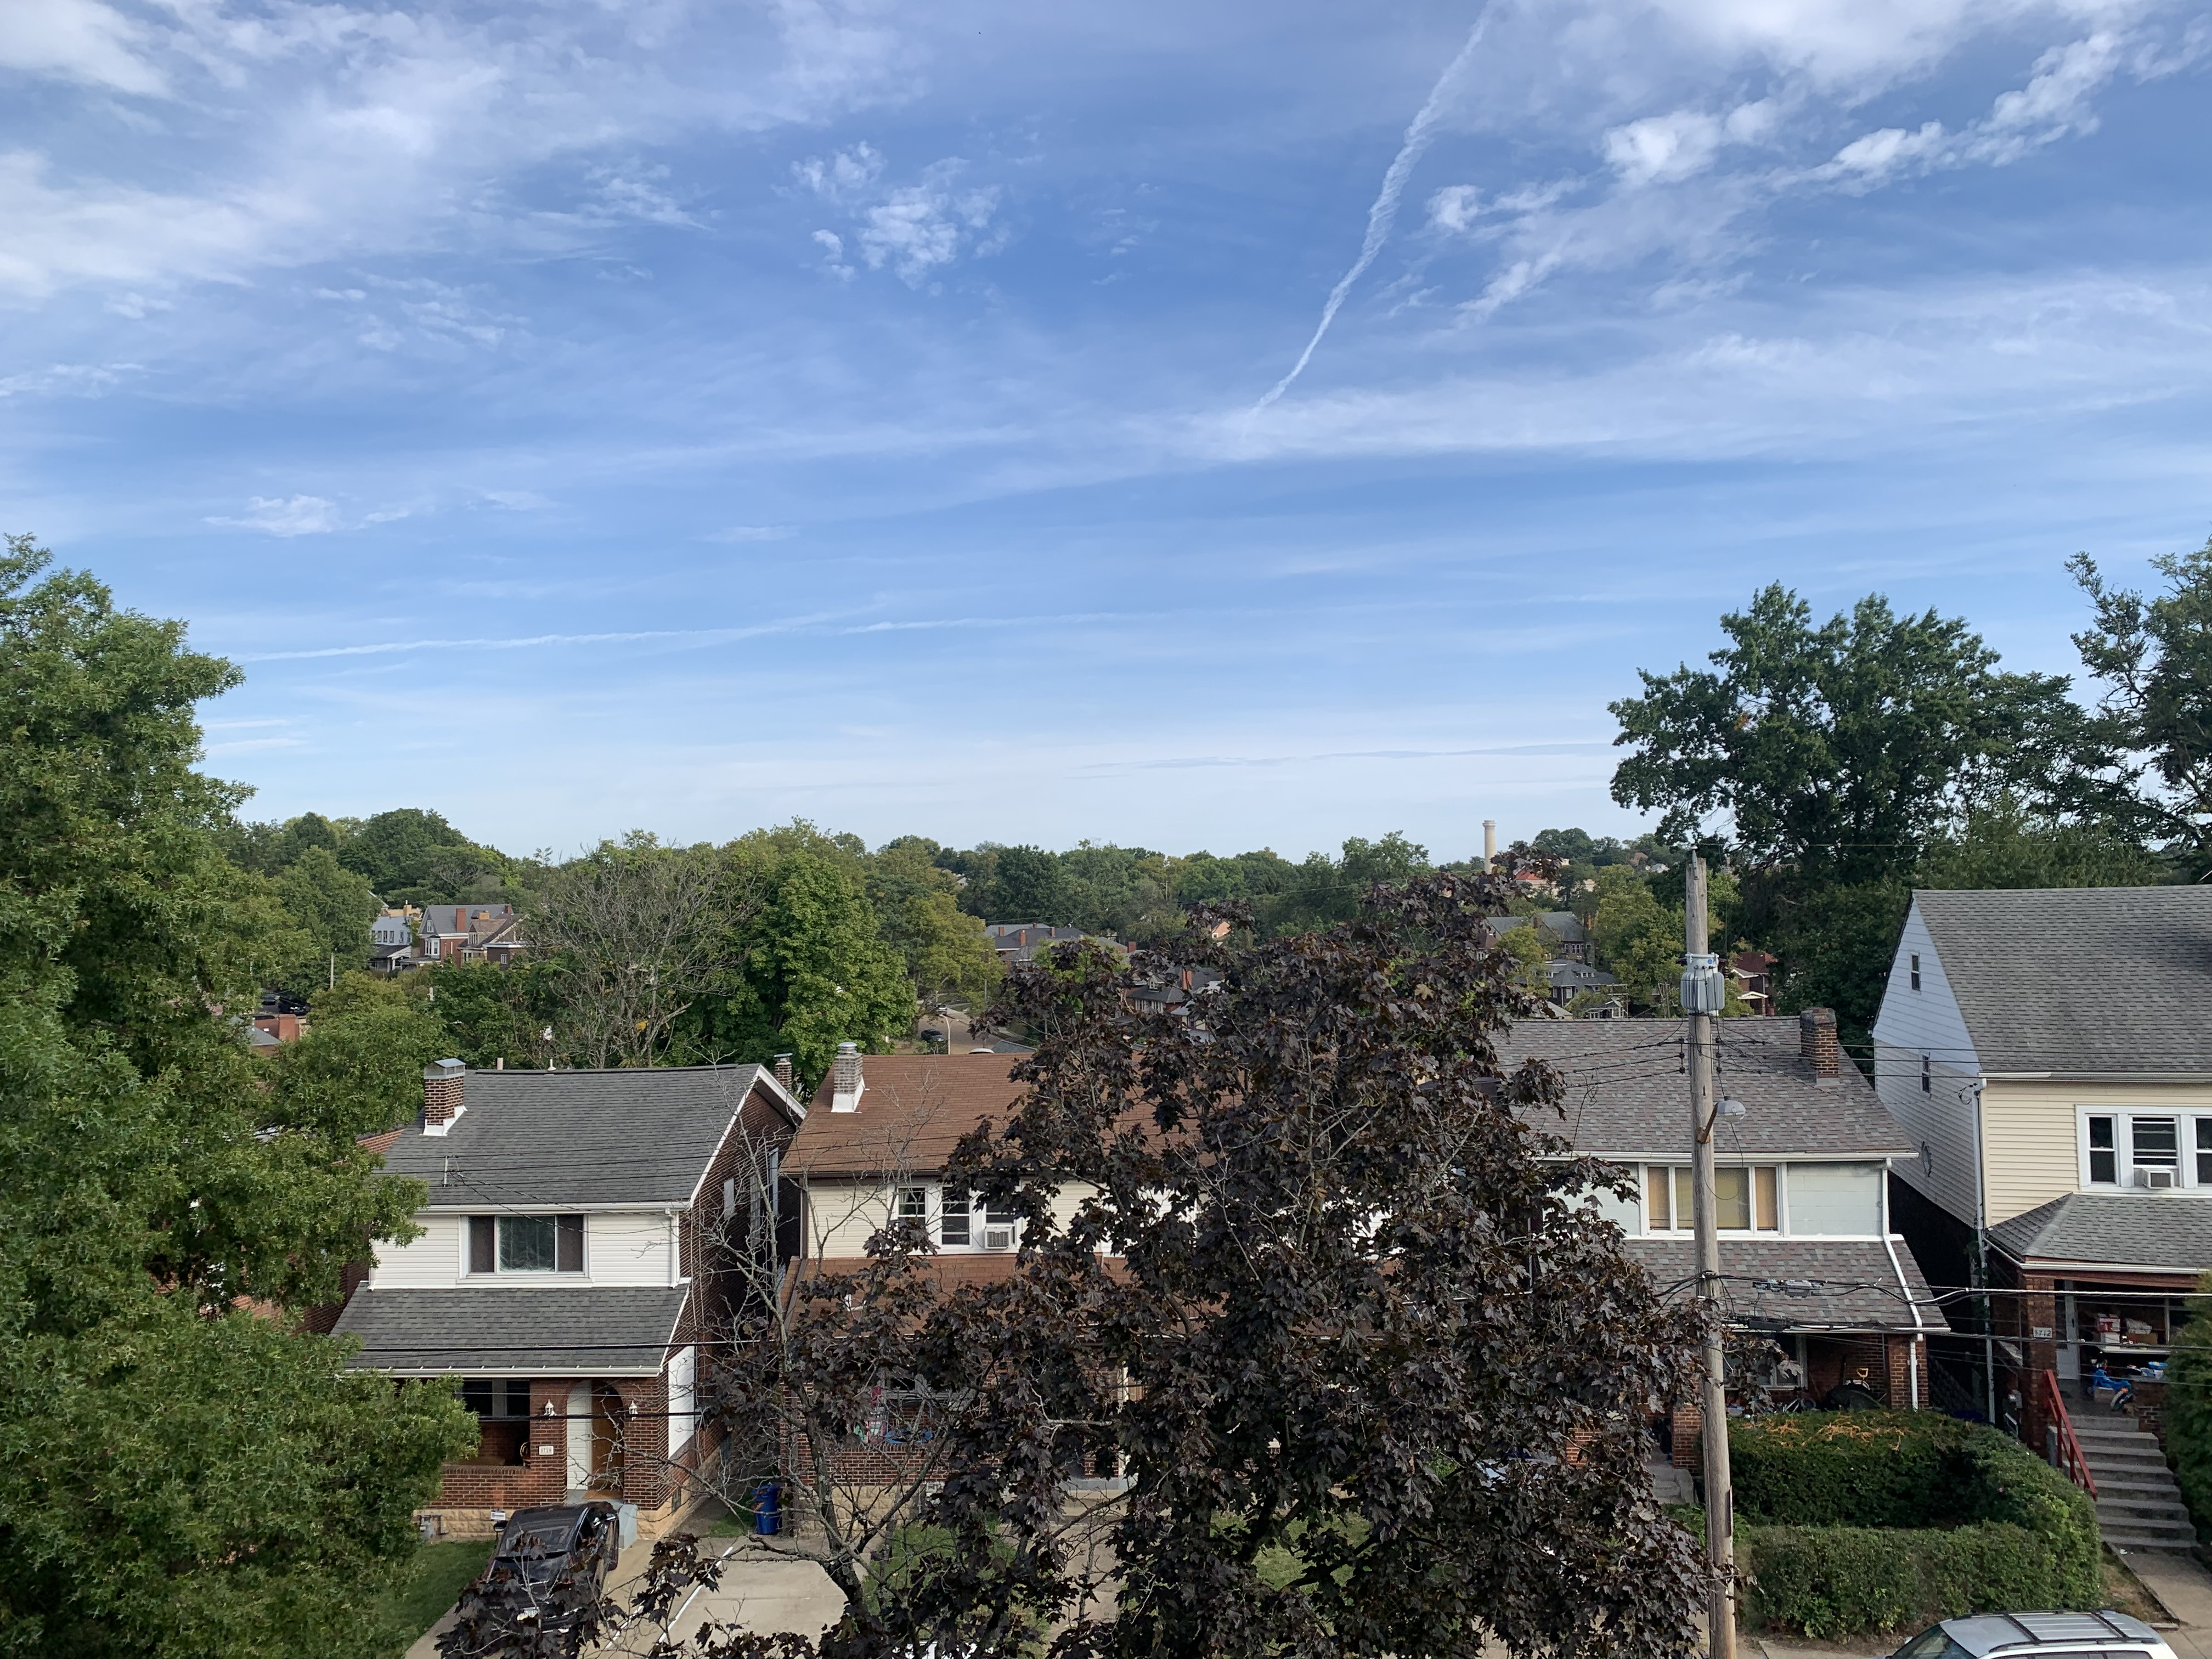
\includegraphics[width=\textwidth]{./data/my_pano_left.jpg}  % Replace with your image file
		\caption{Q4. My Input Left Image}
		\label{fig:Q4_input_left_img}
	\end{minipage}
	\hfill  % This adds space between the images
	\begin{minipage}[b]{0.45\textwidth}
		\centering
		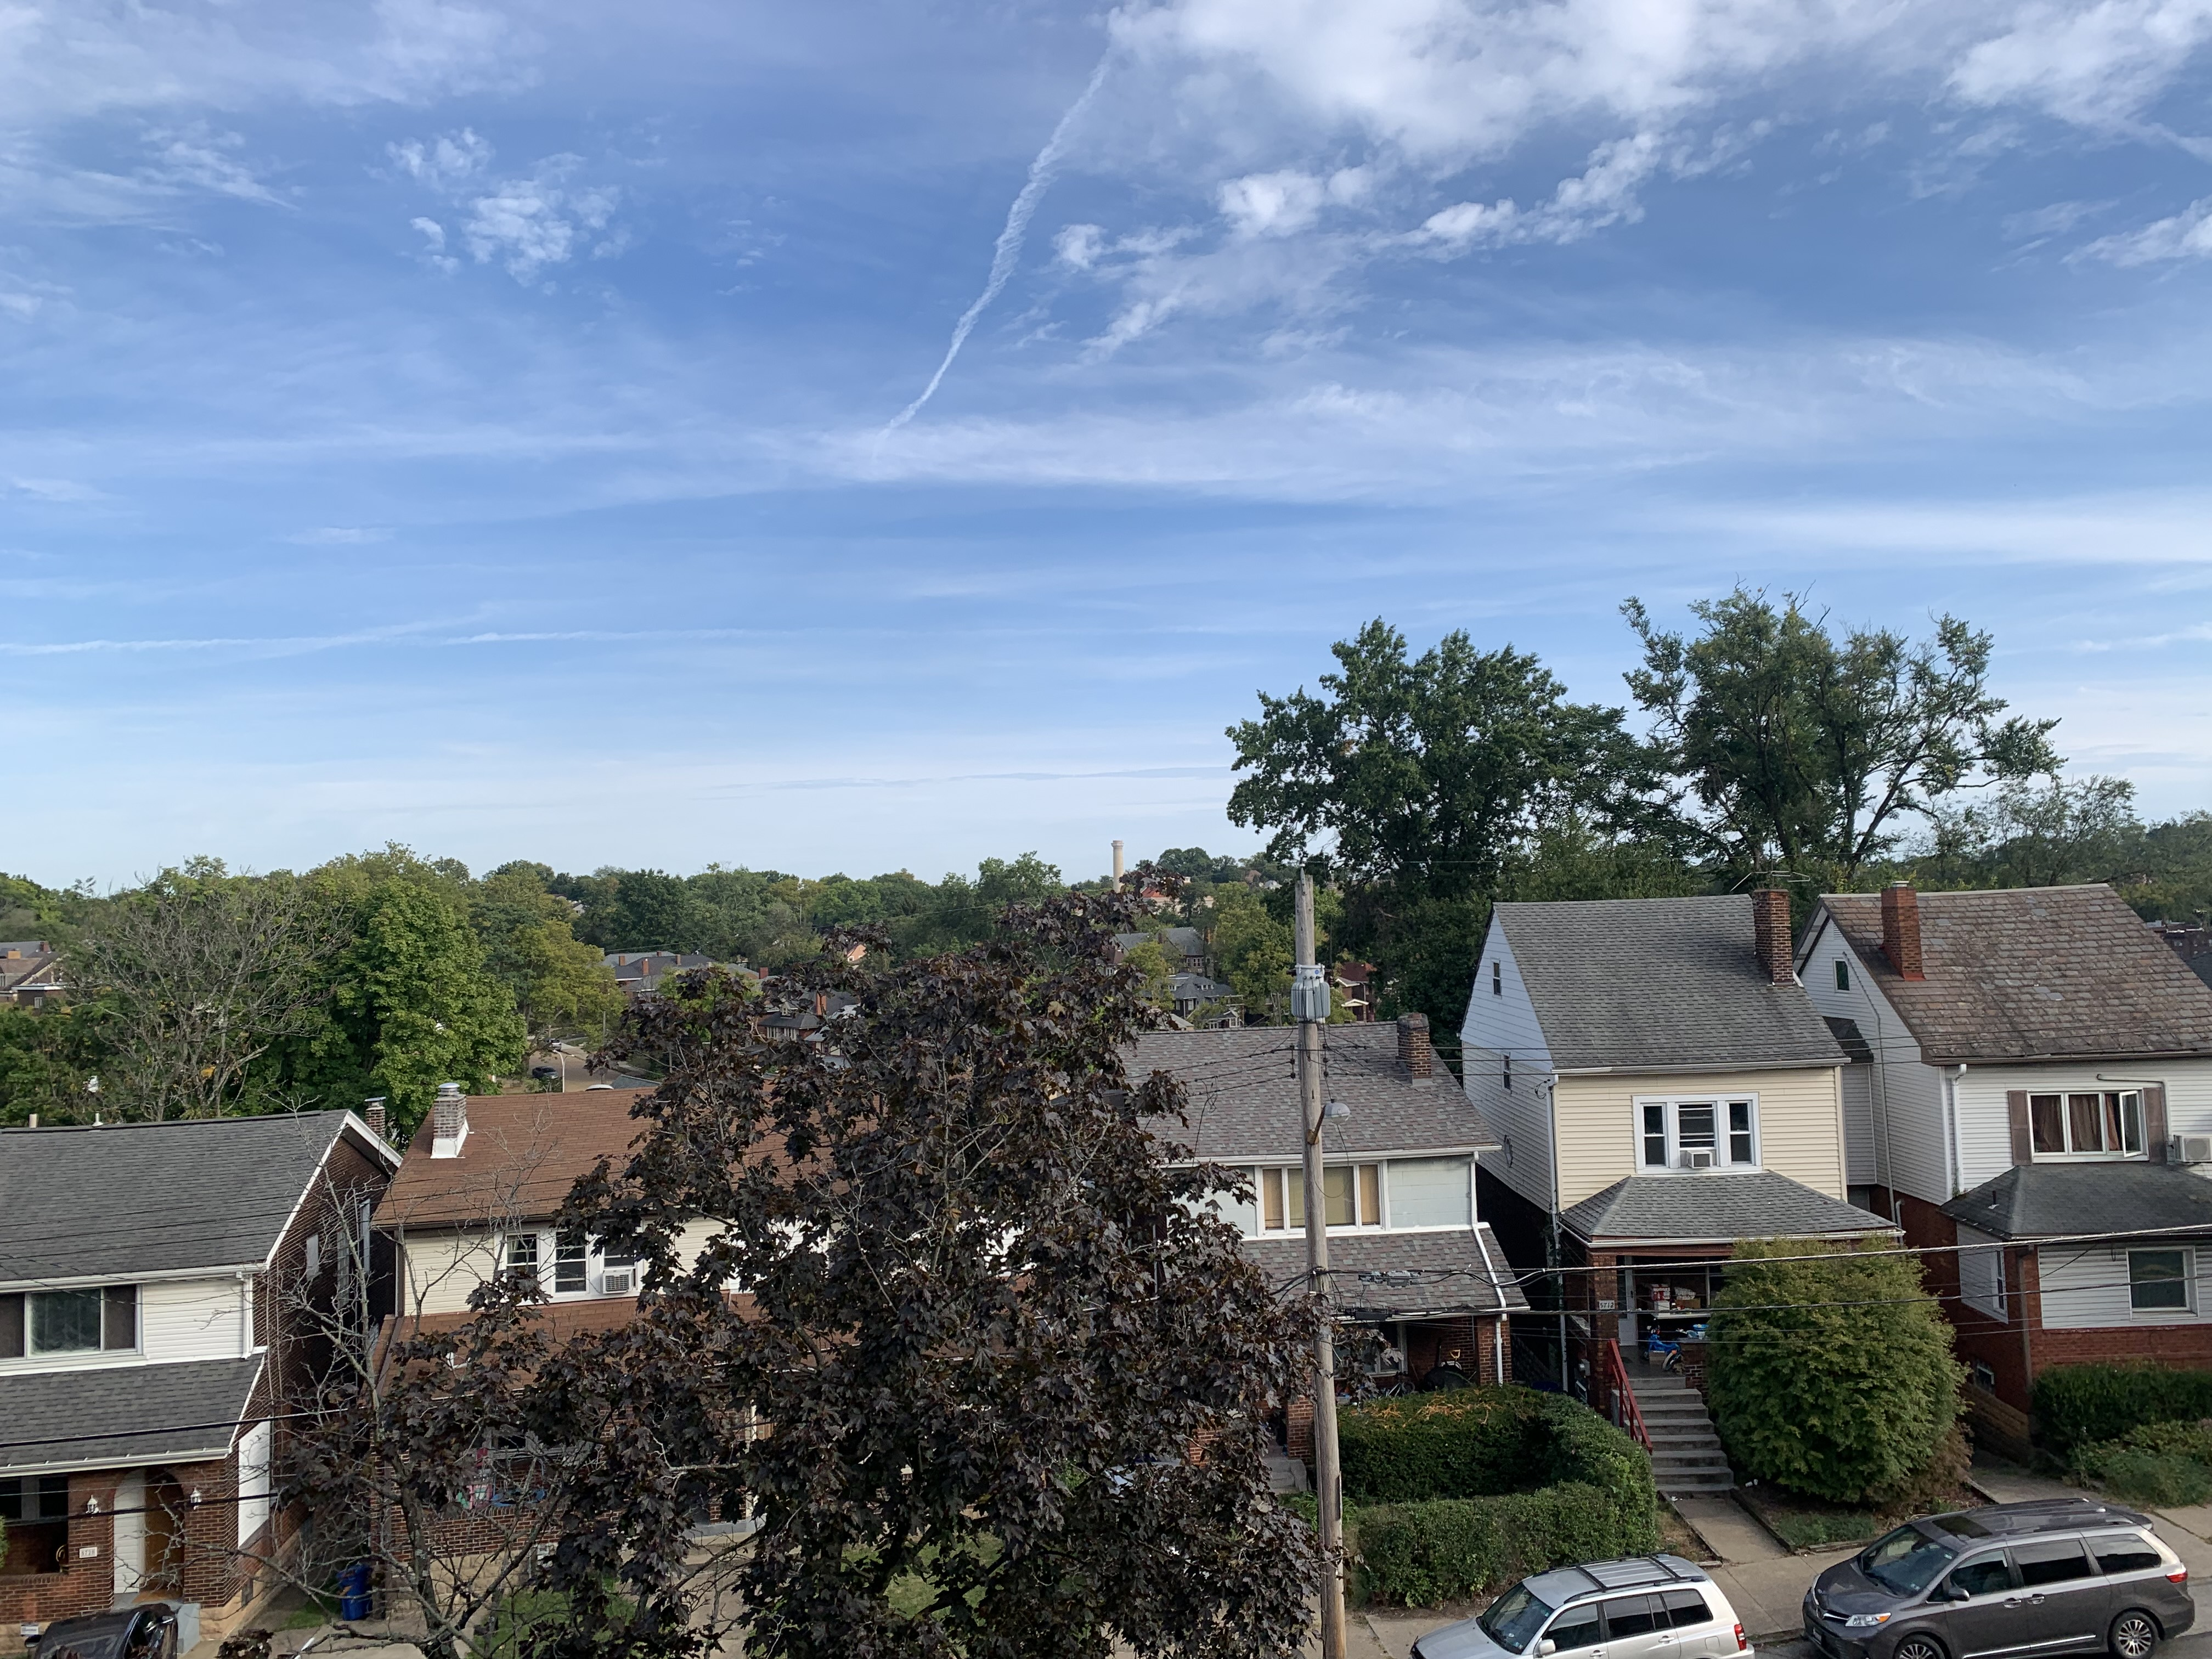
\includegraphics[width=\textwidth]{./data/my_pano_right.jpg}  % Replace with your image file
		\caption{Q4. My Input Right Image}
		\label{fig:Q4_input_right_img}
	\end{minipage}
	\end{figure}
	\begin{figure}[H]
		\centering
		\includegraphics[width=\textwidth]{./result_panorama/Q4_Panorama_Result.png}  % Replace with your image file
		\caption{Q4. Result of Panorama}
		\label{fig:Q4_result_pano}
	\end{figure}	

	\begin{figure}[H]
		\centering
		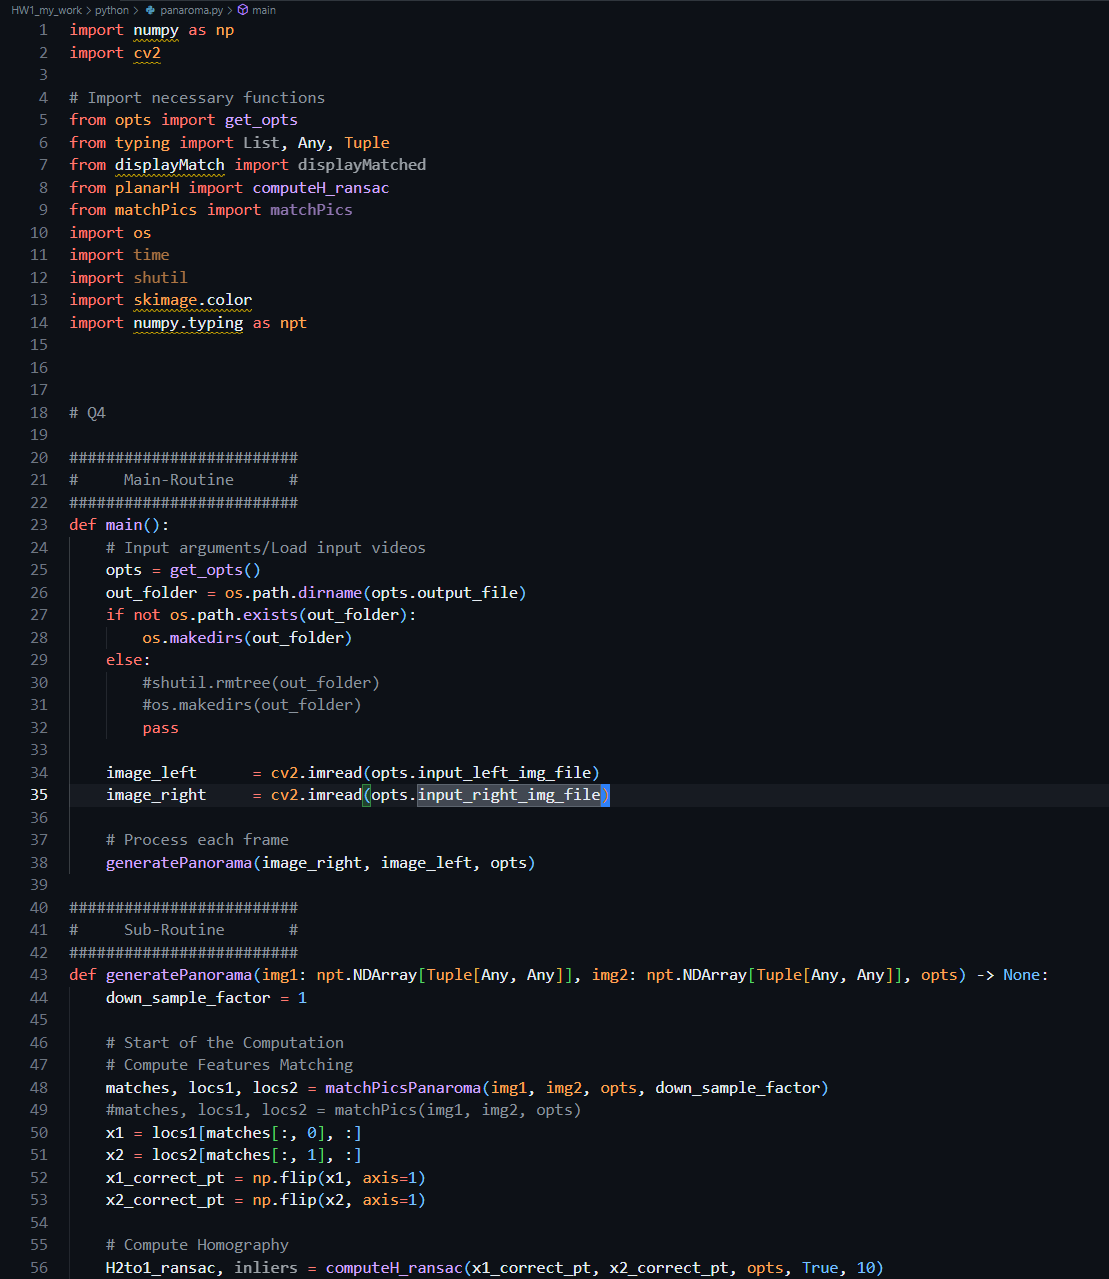
\includegraphics[width=0.7\textwidth]{./Q4_pano_cns1.png}  % Replace with your image file
		\caption{Q4. Code Snippet 1}
		\label{fig:Q4_cns1}
	\end{figure}
	\begin{figure}[H]
		\centering
		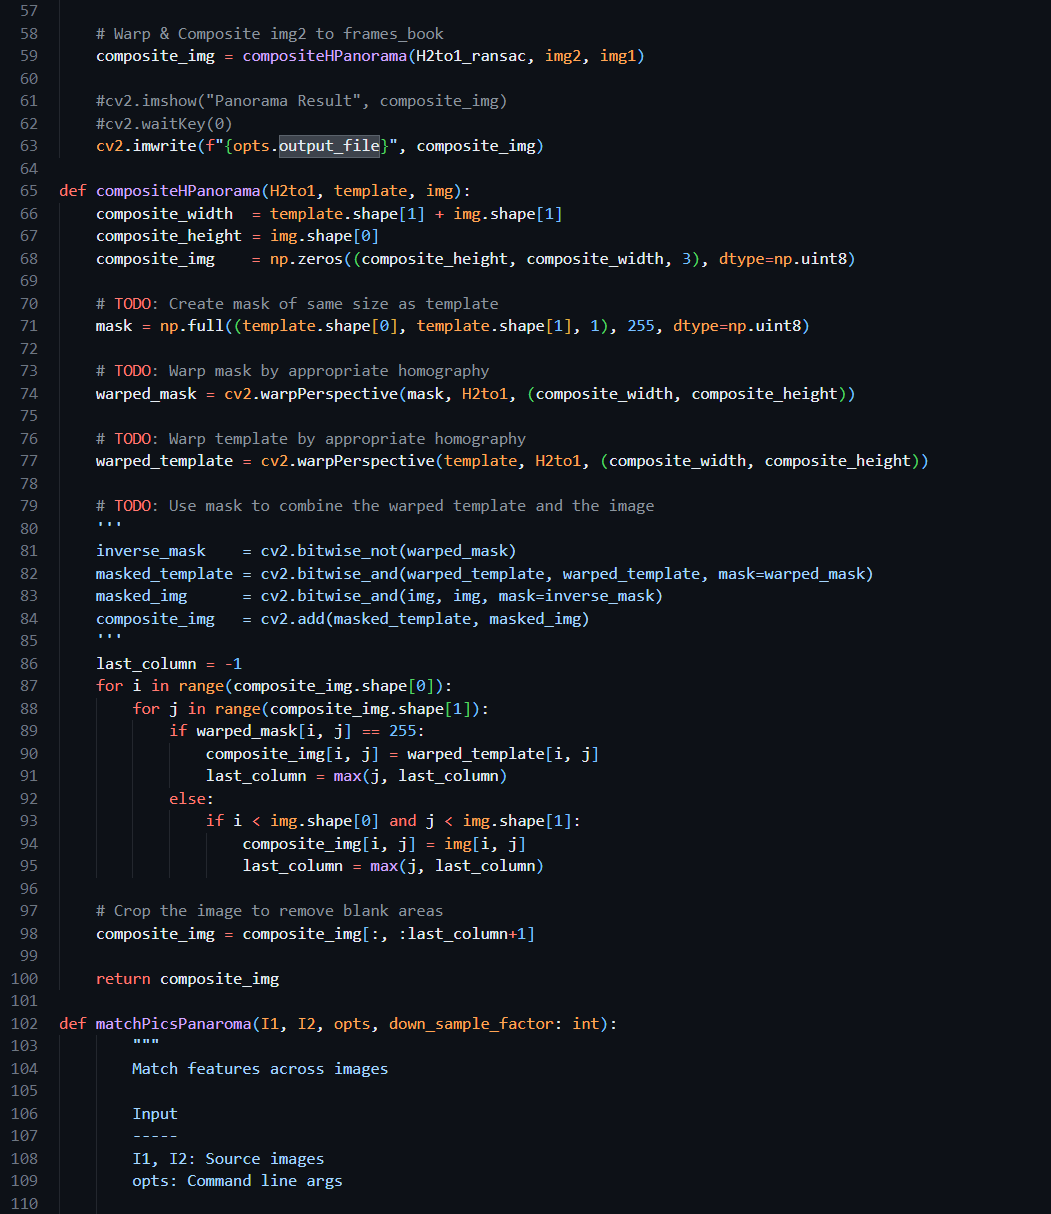
\includegraphics[width=0.7\textwidth]{./Q4_pano_cns2.png}  % Replace with your image file
		\caption{Q4. Code Snippet 2}
		\label{fig:Q4_cns2}
	\end{figure}	
	\begin{figure}[H]
		\centering
		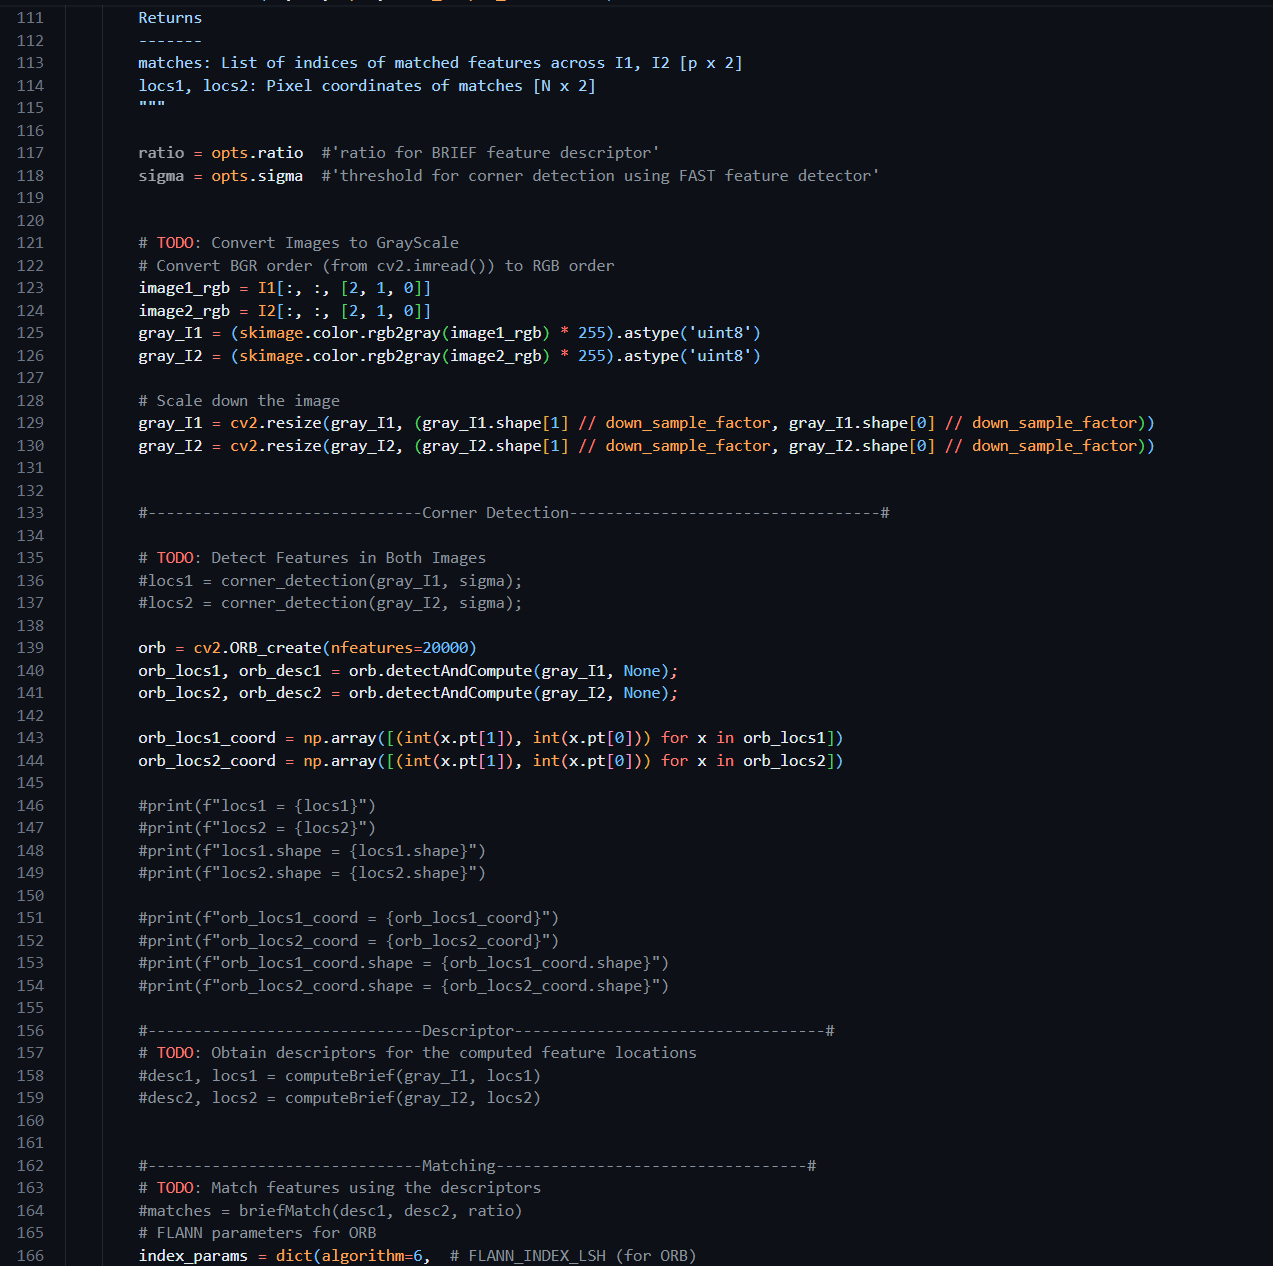
\includegraphics[width=0.7\textwidth]{./Q4_pano_cns3.png}  % Replace with your image file
		\caption{Q4. Code Snippet 3}
		\label{fig:Q4_cns3}
	\end{figure}	
	\begin{figure}[H]
		\centering
		\includegraphics[width=0.7\textwidth]{./Q4_pano_cns3.png}  % Replace with your image file
		\caption{Q4. Code Snippet 3}
		\label{fig:Q4_cns3}
	\end{figure}

	
\end{document}